% Draft #2
\documentclass[12pt,a4paper,twoside,openright]{report}
\usepackage[pdfborder={0 0 0}]{hyperref}  % turns references into hyperlinks
\usepackage[margin=25mm]{geometry} % adjusts page layout
\usepackage{graphicx} % allows inclusion of PDF, PNG and JPG images
\usepackage{import}
\usepackage{docmute}  % only needed to allow inclusion of proposal.tex
\usepackage[sorting=none,backend=bibtex]{biblatex}
\usepackage[super]{nth}
\usepackage{subfig}
\usepackage{array}
\usepackage{booktabs}

% \usepackage{showkeys}

\usepackage{amsmath}
\usepackage{amsthm}
\usepackage{txfonts}
\usepackage{lmodern}
\usepackage{proof}
\usepackage{mathtools}
\usepackage{enumitem}
\setlistdepth{20} % Magically makes the 'too deeply nested' error go away on some cases
\usepackage{array}

\usepackage{listings}
\usepackage{verbatim}
\usepackage{minted}
\usepackage{thmtools}
\usepackage{etoolbox}

\theoremstyle{definition}
\newtheorem{definition}[equation]{Definition}

\newtheoremstyle{dotless}{\topsep}{\topsep}{\itshape}{}{\bfseries}{}{5pt plus 1pt minus 1pt}{}
\theoremstyle{dotless}
\newtheorem{lemma}[definition]{Lemma}
\newtheorem{theorem}[definition]{Theorem}


\bibliography{mybib}
\raggedbottom
\sloppy
\clubpenalty1000%
\widowpenalty1000%

\usemintedstyle{friendly}
\newcommand*{\js}{\mintinline{javascript}}
\newcommand*{\orig}{\ensuremath{\!\multimapinv\!}}

\usepackage{float}
\makeatletter
\newcommand\fs@plainruled{\def\@fs@cfont{\rmfamily}\let\@fs@capt\floatc@plain%
  \def\@fs@pre{}%
  \def\@fs@mid{\kern2pt\hrule\vspace\abovecaptionskip\relax}%
  \def\@fs@post{}%
  \let\@fs@iftopcapt\iffalse
}
\patchcmd{\@thm}{\trivlist}{\list{}{ \leftmargin=1.5em}}{}{}
\patchcmd{\@endtheorem}{\endtrivlist}{\endlist}{}{}
\makeatother
\floatstyle{plain}

\declaretheoremstyle[
spaceabove=6pt, spacebelow=6pt,
headfont=\normalfont\bfseries, numbered=no,
notefont=\textsc, headpunct={\\}, notebraces={}{},
bodyfont=\normalfont,
postheadspace=1em
]{casestyle}
\declaretheoremstyle[
spaceabove=6pt, spacebelow=3pt,
headfont=\normalfont\bfseries,
notefont=\scshape, headpunct={}, numbered=no,
bodyfont=\normalfont,
postheadspace=1em
]{subcasestyle}
\declaretheorem[style=casestyle]{case}
\declaretheorem[style=subcasestyle, name=case]{subcase}

\setlength\partopsep{-\topsep}
\addtolength\partopsep{-\parskip}
\usepackage{chngcntr}
\newfloat{program}{thp}{lop}[chapter]
\AtBeginDocument{\counterwithin{listing}{chapter}}
\floatname{program}{Listing}
\usepackage{tabu}
\usepackage{adjustbox}
\newcommand{\myinfer}[3]{%
  $\infer[\footnotesize\textsc{#1}]
  {#2}{
	{
	  \renewcommand{\arraystretch}{0.9}
	  \begin{tabular}{>{$}c<{$}}
		#3	
	  \end{tabular}
	}
  }$
}
\newcommand{\infertable}[1]{%
  \begin{table}[H]
  	\centerline{
  	  \begin{adjustbox}{max width=\linewidth,center}
	  	\begin{tabular}{c c}
		  #1
	  	\end{tabular}%
  	  \end{adjustbox}
  	}
  \end{table}
}
\usepackage{xcolor}
\definecolor{mintedbackground}{rgb}{0.95,0.95,0.95}

\newminted[jscript]{javascript}{
bgcolor=mintedbackground,
fontfamily=tt,
linenos=true,
numberblanklines=true,
numbersep=-12pt,
gobble=0,
frame=leftline,
framerule=0.4pt,
framesep=2mm,
funcnamehighlighting=true,
tabsize=4,
obeytabs=false,
mathescape=true
samepage=false, %with this setting you can force the list to appear on the same page
showspaces=false,
showtabs =false,
texcl=false,
}
\renewcommand{\baselinestretch}{1.1}  % adjust line spacing to make more readable
\newcommand{\typable}[2][ ]{\Gamma{}\vdash\mathtt{#2}\, |_C#1\:\Gamma#1'}
\newcommand{\typed}[2]{\Gamma{}\vdash\mathtt{#1}: #2\,|_C\:\Gamma'}
\newcommand{\transition}[6]{\langle{}\mathtt{#1},#2,#3\rangle{}\rightarrow{}\langle{}\mathtt{#4},#5,#6\rangle}
\newcommand{\indHyp}{\Phi(\Gamma, m, C, \Gamma')}
\newcommand{\indHypTwo}{\Psi(\Gamma, e, T, C, \Gamma')}
\newcommand{\var}{\textbf{var}}
\newcommand{\sub}[1]{\textsubscript{#1}}
\newcommand\eqdef{\mathrel{\overset{\makebox[0pt]{\mbox{\normalfont\tiny def}}}{=}}}
\newcommand\qdot{\mathbin{\scalebox{1.5}{.}}\enspace}
\begin{document}






\chapter{Introduction}\label{introduction}

Types are a way of grouping together values which support similar operations.
For example, \texttt{number} might be a type representing values which support
addition and subtraction. \texttt{string} might represent a sequence of
characters which supports concatenation, but doesn't support addition or
subtraction. A program in a language with these types cannot subtract a
\texttt{number} from a \texttt{string}, and an attempt to do so is known as a
\textit{type error}. We say that a language is \textit{strongly} typed if such
attempts will always generate some kind of error, whereas a \textit{weakly}
typed language may allow the operation to execute, with sometimes
unpredictable consequences. Under \textit{dynamic} typing, checking for type
errors happens at the very last minute -- during program execution itself.
Using a \textit{static} type checker, the program code can be analysed in
advance to identify type errors before the program runs.

JavaScript is a high-level, dynamically-typed programming language which was
originally designed for little more than validating forms on websites. Today
the language is an essential part of everyday computing, powering demanding
online applications such as image editors, IDEs and online games. The
execution context of the language has also changed, moving from the browser to
the server, and now even being targeted by other languages'
compilers~\cite{asm}. As the scale of JavaScript applications has increased,
so too has the complexity of development projects. Assurance that a program is
bug-free has become more critical, both for online companies which rely on
JavaScript for e-commerce, and for the people who use their applications. A
security bug in an online banking application, for example, could be
devastating. JavaScript's weak typing discipline, however, makes it hard to
reason about a program's correctness, and limits the information available to
development tools. This problem is exacerbated by JavaScript's type
\textit{coercion}, which permits expressions which would normally be deemed
untypable by, for example, converting any object to the value \js{true} when
placed in a context expecting a boolean. This can result in the silent propagation
of type errors, providing no explicit errors to the developer.

Static type checking catches potential bugs earlier in the development cycle,
and can allow programs to run faster, without needing to check types before
every operation. However, it is impossible for a static type checker to
precisely identify all potential type errors, because it cannot know what the
program's behaviour will be when it runs. If such a type checker did exist, it
could be used to determine whether any given program will terminate or not --
which would violate the undecidability of the halting problem. Instead, a
conservative approximation is made, and some programs which would never
actually exhibit a type error will fail a static type check. This approximation
can be frustrating for developers, who will need to satisfy the type checker by
rewriting their code before it will run.

Although languages are often described as being statically or
dynamically-typed, in reality it is compilers and interpreters which enforce a
particular discipline. A compiler for a traditionally statically-typed language
could skip the static type checking phase and insert dynamic type checks
instead. In the other direction, it is sometimes possible to perform static
analysis of a program's code in order to avoid reliance on delayed runtime
checks.

Several such attempts have been made to perform static analysis on JavaScript,
which is typically a dynamically-typed language. ECMAScript~4~\cite{es4},
a proposed extension to the JavaScript standard, featured optional type
annotations, but the proposal was never finalised and the annotations are not
present in later versions of the standard. TypeScript~\cite{ts}, uses a
superset of JavaScript syntax with similar annotations, and compiles this back
into JavaScript. These approaches have depended on programmer-inserted type
annotations, which limit their utility for legacy codebases. Some projects
have attempted to use Hindley-Milner style analysis to infer the types of
program expressions automatically~\cite{anderson06, tajs, guha}, including the most
recent contribution, Flow~\cite{flow}. 

Any static analysis, however, will struggle to offer reliable results because
of the inherently dynamic nature of the language. Many traditional JavaScript
programming idioms are legitimately untypable. JavaScript has no
mechanism for overloading functions, for example, so many developers write
functions expecting different parameter types from call-to-call, and use manual
type checks to handle them (see Listing~\ref{lst:dynamicIdiom}). Flow and
TypeScript allow for untypable functions using a special `any' type, which will
never trigger a static type error. The obvious disadvantage here is that the
static analysis can no longer make any guarantees about the soundness of the
program, as certain parts of it have effectively not been checked.
\begin{program}[t]
  \begin{jscript}
 	// adapted from the Prototype library
 	function serialize(val) {
	  switch (typeof val) {
		case "boolean":
		return val ? "true" : "false";
		case "number":
		return "" + val;
		case "string":
		return val;
	  }
 	}	
  \end{jscript}
  \caption{Dynamic idioms in JavaScript}
  \label{lst:dynamicIdiom}
\end{program}
Additionally, JavaScript code rarely operates in isolation in modern web
applications. Even if a program passes the static type checker, some external
piece of code may introduce a type error by, for example, passing data of the
incorrect type to a well-typed function.

Gradual typing is a technique used to make safety guarantees about code which
combines both static and dynamic typing. Initially looking at interoperation
between static and dynamic languages~\cite{gray2005fine}, the concepts are
also applicable here, where the division between static and dynamic code lies
within one language rather than between several. Since static analysis cannot
guarantee that the program is free of dynamic type errors, we instead
guarantee that only dynamic properties of the code are able to cause runtime
errors -- that the well-typed code ``can't be blamed"~\cite{cantblame} for
any type errors which arise. This is achieved by protecting the boundaries
between the type-safe and type-unsafe `worlds'. Conversions are made from the
dynamic values, and although this conversion process may
generate an error (for example trying to convert a \texttt{number} to a
\texttt{string}), the type safety of the well-typed world is provably
preserved.

In this project, I have defined a formal operational semantics and a type
system for a subset of JavaScript, and created a proof that the system defined
has the properties of \textit{progress} and \textit{type preservation}. I have
successfully implemented type inference according to this specification in
order to create a static type checker, and this implementation has been checked
by a large suite of tests. In doing this, I realised that the subset of
JavaScript initially planned to be supported was insufficient for `real-world'
code, and added arrays and object growth to both the specification and
implementation. This enabled me to test my implementation using five tests from
the Mozilla SunSpider JavaScript benchmark suite. Finally, I integrated ideas
from research in the field of gradual typing to allow type-checked code to
inter-operate safely with unchecked code. The only extension task left
incomplete is the inclusion of object inheritance via object prototypes, but I
present a starting point to this, which could fruitfully be built upon in
future work.

\begin{figure}
  \centering
  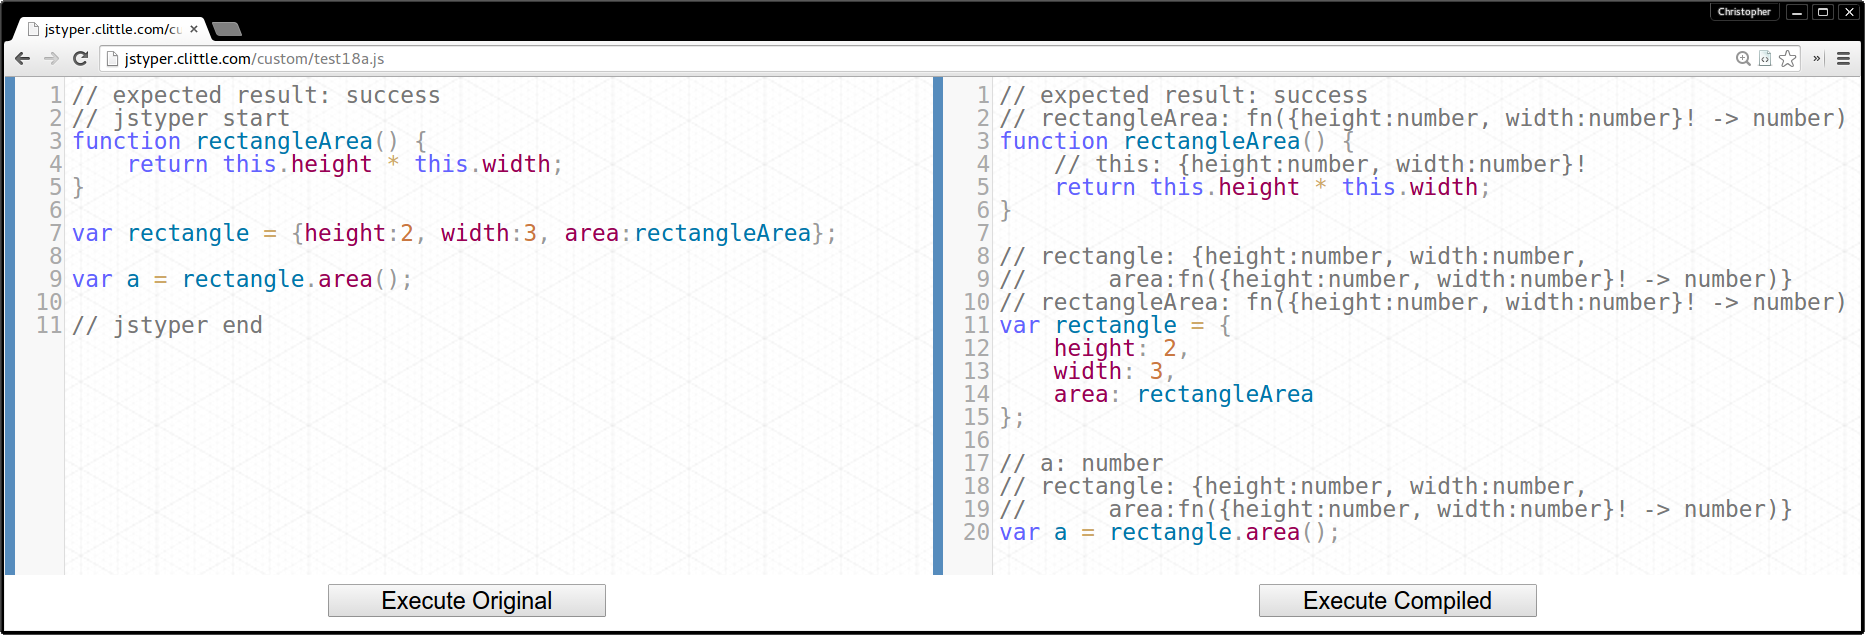
\includegraphics[width=160mm]{../res/web-interface.png}
  \caption{The web interface to my type inference system. Annotations are inserted as comments indicating the 
  	types of any variables which occur in the succeeding line.}
  \label{fig:web-interface}
\end{figure}






\chapter{Preparation}\label{preparation} 
\section{Background}

Before development could begin, an understanding of the theoretical
underpinnings of the project was required. Several of the undergraduate courses
offered as part of the Tripos were a valuable introduction, notably the Part IB
course \textit{Semantics of Programming Languages}, and the Part II courses
\textit{Types} and \textit{Optimising Compilers}. \textit{Semantics of
  Programming Languages} introduced the proof techniques necessary for proving
type soundness, but for an insufficiently complex example language to cover all
strategies required. Pierce's \textit{Types and Programming
  Languages}~\cite{pierce} bridged this gap sufficiently that I was able to look
at recent work defining the operational semantics of real dynamic programming
languages~\cite{pythonOpSem}. The \textit{Types} course similarly introduced
the Hindley--Damas--Milner algorithm for type inference, and Pierce's book
helped develop those ideas further. Neither course touched on the topic of
gradual typing, which is very much a topic of current research interest. A few
papers by Siek~\cite{gradSiek, gradSiek2} and Gray~\cite{gradGray} proved
sufficiently accessible, however, for me to explore the area.
\textit{Optimising Compilers} presented techniques for control flow analysis,
which usefully complement the inference-based analyses, for example by checking
that a variable has been defined before use.

I began the project with a strong informal grasp of the JavaScript language.
JavaScript implementations are guided by the ECMAScript
specification~\cite{ecmaSpec}, which offered a more rigorous definition,
required to define my own operational semantics. Some work has already been
done attempting to formalise the semantics of
JavaScript~\cite{guha2010essence}, providing useful inspiration in designing my
own operational semantics. 

Carrying out any kind of static analysis on a dynamic language will result in
false negatives, where a safe statement is incorrectly deemed unsafe. This is
preferable to a false positive in terms of guaranteeing safe operation of the
program, but still frustrating for the developer. It can be important,
therefore, to understand the manner in which a language is actually used. There
is little benefit in devising solutions to the problem of typing dynamic idioms
which are hardly ever used, and so I looked through the results of Richards,
Lebresne, Burg and Vitek~\cite{JSBehaviour}, who have analysed the dynamic
behaviour of real JavaScript programs in operation on the internet. It
was educational to look at TypeScript~\cite{ts,understandingTS}, to learn from
the design decisions which had been made, the solutions they had already found,
and to fully understand the limitations of their solution. I also attended a
talk on Flow by one of the authors, with similar ambitions.

\section{Development Plan}

The project consisted of four discrete tasks: designing a formal specification
to describe the operational semantics and type judgements for my subset;
proving that the subset as specified was sound and implementing both the type
inference system and the gradual typing compiler. Orthogonally to this
separation of tasks, the language was divided into discrete features, such as
if-statements, binary operations and loops. This division meant the project
lent itself to an incremental build model, whereby each build increment
introduced a new language feature to the specification, proof and
implementations. This allowed development to proceed systematically, offering
sensible opportunities for regression testing after each iteration, with only
few changes since the last test. This strategy also minimised development risk
by allowing me to cease development at the end of any iteration and still have
a successful system, albeit supporting fewer features than planned.

I used Git for version control, with the primary repository hosted on GitHub
also serving as a remote backup of my work. To amplify the benefit of my
regression tests for bug detection, I set up continuous integration such that
each time the GitHub repository was updated, the code was downloaded to a
private VPS, and the full test suite run automatically. If any tests failed, an
email warning was sent to me, so I was immediately alerted of the problem I had
introduced, and could fix it while the changes which had triggered it were
still fresh in my mind. If all tests passed, the new code was deployed to a web
server, such that a live demo was always accessible online.\footnote{
  \href{http://jstyper.clittle.com}{http://jstyper.clittle.com}}

Within each iteration, I began with the specification.
The specification was written using
Ott~\cite{sewell2007ott}, a tool which I learnt to use as the project
progressed. The iteration would be considered complete when each of the other
components conformed to the specification. For the two development tasks, I
proceeded in a test-driven manner, whereby I would first write tests involving
the new language feature, expecting them to fail. Development then aimed to
make these failing test-cases pass. My collection of tests available for
regression testing (and later for benchmarking) thus grew consistently across
the project life-cycle, and by the end of the project 
\input{|"ls ../../src/tests/custom/results -l | wc -l"}such tests had been produced.

Many developers view theoretical computer science as carrying little practical
benefit for them, when the truth is that concrete implementations of the theory
can bring huge practical benefits. It was thus important to me to integrate
smoothly within the existing JavaScript ecosystem rather than enforce a
non-standard workflow for JavaScript developers. This would reduce the barriers
to entry and make the advantages of static typing more easily discoverable to
those who would most benefit from it. Languages like OCaml, although commonly
used for this kind of project within the academic community, are less likely to be
present on a web developer's computer. Indeed, this is a problem Chaudhuri
mentioned having for Flow, which has been released as an open source project
but suffers from a lack of contributors because the project's main users are
not able to understand or make meaningful contributions to code base.
Instead, I decided to write the type inference system in JavaScript, thus
ensuring it could run on any system. This decision opened the door for writing
a self-hosting compiler, which could type-check and compile its own source
code. It also potentially made it possible for type checking and compilation to
happen in the browser, though in practice this would likely only be advantageous in
fairly unusual circumstances. Instead, development focussed on running the
compiler using Node.js~\cite{nodejs}, a JavaScript interpreter designed for use
outside the browser.

As an interpreted language, JavaScript is not compiled prior to execution, but
it is often compressed to speed up download times to client computers. A number
of static analysis tools exist to aid with this, performing mainly control-flow
analyses to, for example, eliminate unused variables from the source code
(known as \textit{minification}). Although I was not interested in such
analyses, it seemed sensible to integrate with a standard abstract syntax tree
(AST) format, and use existing parsing and code-generation solutions.
UglifyJS\footnote{\href{http://lisperator.net/uglifyjs}{http://lisperator.net/uglifyjs}} is one of the
most-used minification libraries for JavaScript, and has separate components
for parsing and code generation but uses a custom (albeit well-documented) AST
format. Esprima\footnote{\href{http://esprima.org}{http://esprima.org}} is another JavaScript parser
which is marginally faster and uses the SpiderMonkey AST format standardised by
Mozilla. Various analysis tools and code generators exist for this format, but
I decided that the UglifyJS format was actually more useful for my purposes,
and parse speeds was not a priority. For example, the SpiderMonkey AST has a
single representation of any unary expression, when in practice it can be
useful to distinguish between prefix and suffix expressions.  Additionally,
UglifyJS uses object inheritance to define its node types, where Esprima
prefers flat objects. 




\chapter{Implementation}\label{implementation}

There were three components to implement for the project -- the formal
specification of the language; the executable type inference system itself and
a gradual typing compiler to protext the boundaries of the typed world.  The
language I specified was a subset of JavaScript, chosen to be expressive enough
to represent actual JavaScript programs while being free of some of the
complications of implementation. For example, storage of variables was
simplified to just a scope and a heap, without modelling the special cases of
the global scope, nor worrying about removal of unused data by the garbage
collector. 

\section{Language Definition}

The subset chosen includes primitive constants; object and array literals;
arithmetic and logical binary and unary operators; dereferencing from and
assignment to object properties and array elements; functions and function expressions; and basic control flow via \js{if ... else ...} and loops.  
Where features of JavaScript were omitted, they largely tended to be features
which could be desugared into supported features -- for example \js{switch}
statements can be written as a series of \js{if} statements, and do not present
an interesting problem from a typing perspective. No attempt was made to
include a representation of commonly used JavaScript objects, such as the
\js{RegExp} object or elements of the \textit{Document Object Model}, which is used to
represent the structure of an HTML document. The type signatures of such objects
could be predefined for use within the system.

Some other features were excluded which would introduce difficult problems in
ensuring type safety.  Although I included the ability to dynamically grow an
object by assigning to an undefined property, I excluded the ability to remove
or change properties once defined. These features, although legal in
JavaScript, make it difficult to reason about the type safety of a property
access without control flow analyses keeping track of precisely which
properties are well-defined at each program point. Another example is the
concatenation of strings using \js{+}, which overloads the use of the \js{+}
operator to represent more than one method signature. Even where a feature is
missing, however, the gradual typing mechanism usually allows code fragments
relying on these features to bypass the type checker.

\begin{listing}
  \begin{lstlisting}[mathescape, escapechar=£,caption={Language Definition},label={lst:langdef}]
v            ::= $b$ | $n$ | $str$ | £\textbf{undefined}£ | £\textbf{null}£
                    | £\textbf{\{}£$l_1$:$v_1$, $\dots$, $l_i$:$v_i$£\textbf{\}}£ | £\textbf{[}£$v_1$, $\dots$, $v_i$£\textbf{]}£ | £[\![£$func$, s£]\!]£
e            ::= $v$ | $id$ | $e$ $op$ $e'$ | £\textbf{\{}£$l_1$:$e_1$, $\dots$, $l_i$:$e_i$£\textbf{\}}£ 
                    | £\textbf{[}£$e_1$, $\dots$ $e_i$£\textbf{]}£ | $e$£\textbf{.}£l | $e$£\textbf{[}£$e'$£\textbf{]}£ 
                    | $e$£\textbf{(}£$e_1$, $\dots$, $e_i$£\textbf{)}£ | $func$
                    | $assignTarget$ $\approx$ $e$ | $assignTarget$ $assignOp$ 
                    | $assignOp$ $assignTarget$ | $preOp$ e
m            ::= $e$ | $m_1$; $\dots$; $m_i$ | £\textbf{var}£ $vd_1$, $\dots$ $vd_i$ 
                    | £\textbf{if}£ £\textbf{(}£$e$£\textbf{)}£ £\textbf{\{}£$m_1$£\textbf{\}}£ | £\textbf{if}£ £\textbf{(}£$e$£\textbf{) \{}£$m_1$£\textbf{\} else \{}£$m_2$£\textbf{\}}£ 
                    | £\textbf{for}£ £\textbf{(}£$e_1$; $e_2$; $e_3$£\textbf{)}£ £\textbf{\{}£$m$£\textbf{\}}£ | £\textbf{for}£ £\textbf{(}£$varDec$; $e_2$; $e_3$£\textbf{)}£ £\textbf{\{}£$m$£\textbf{\}}£ 
                    | £\textbf{while}£ £\textbf{(}£$e$£\textbf{)}£ £\textbf{\{}£$m$£\textbf{\}}£ 
                    | £\textbf{@def function}£ $id$£\textbf{(}£$x_1$, $\dots$, $x_i$£\textbf{)}£ £\textbf{\{}£$m$£\textbf{\}}£
                    | £\textbf{return}£ $e$ | £\textbf{return}£  | £\textbf{$\epsilon$}£
func         ::= £\textbf{function}£ $id$£\textbf{(}£$x_1$, $\dots$, $x_i$£\textbf{)}£ £\textbf{\{}£ $m$ £\textbf{\}}£ 
                    | £\textbf{function}£ £\textbf{(}£$x_1$, $\dots$, $x_i$£\textbf{)}£ £\textbf{\{}£ $m$ £\textbf{\}}£
assignTarget ::= $vRef$ | $assignTarget$£\textbf{[}£$e$£\textbf{]}£ | $assignTarget$£\textbf{.}£l
vRef         ::= $id$ | $vRef$£\textbf{.}£l | $vRef$£\textbf{[}£$n$£\textbf{]}£
vd           ::= $id$ | $id$£\textbf{=}$e$£
op           ::= $numOp$ | $cmpOp$ | $numcmpOp$ | $boolOp$
$\approx$             ::=  £\textbf{=}£ | $numOp$£\textbf{=}£
numOp        ::= £\textbf{+}£ | £\textbf{-}£ | £\textbf{/}£ | £\textbf{*}£ | £\textbf{\%}£
numcmpOp     ::= £\textbf{\textless}£ | $\mathbf{\leq}$ | £\textbf{$\geq$}£ | £\textbf{\textgreater}£
cmpOp        ::= £\textbf{===}£ | £\textbf{!==}£ | £\textbf{==}£ | £\textbf{!==}£
boolOp       ::= £\textbf{||}£ | £\textbf{\&\&}£
preOp        ::= £\textbf{-}£ | £\textbf{!}£
assignOp     ::= £\textbf{-\,-}£ | £\textbf{++}£
  \end{lstlisting}
  \caption{Language Definition}
\stepcounter{program}
  \label{lst:langdef}
\end{listing}

\section{Formal Specification}

The specification of my JavaScript subset has two components -- a definition of
the operational semantics, and a definition of the typing judgement used. The
executable type inference system has the job of verifying that the initial
program, as typed by the developer, is well-typed. If the specification is
correctly defined, this property can then be proven to be preserved throughout the
execution of the program.

\subsection{Operational Semantics}
The operational semantics takes the form of 59 inductive rules
describing all possible transitions from one step of computation to another. A
step of computation is described by a configuration triple of the form
$$\langle \mathtt{m}, s, \theta\rangle.$$ $\mathtt{m}$ is the program code remaining to be
executed, $s$ represents the current scope (the set of variables accessible at
this program point); and $\theta$ represents the heap, where variable values
are stored.


\infertable{
  $\myinfer{Seq2}
  {\langle \mathtt{m_1; m_2; \dots; m_i}, s, \theta\rangle \rightarrow \langle \mathtt{m_1'; m_2; \dots; m_i}, s, \theta\rangle}
  {\langle\mathtt{m_1}, s, \theta\rangle\rightarrow\langle \mathtt{m_1'},s, \theta\rangle}$
}
A transition rule is described by a series of premises, which, if true,
indicate that the conclusion must also be true. For example, the rule
\textsc{Seq2} tells us that, if some statement $\mathtt{m_1}$ can reduce to $\mathtt{m_1'}$ using
the store $(s,\theta)$, then it must also be possible to reduce any sequence of
statements beginning with $\mathtt{m_1}$ with the same effects on the store. Most of the
rules follow an intuitive understanding of JavaScript's execution semantics --
the result of a subexpression is used to determine the type of the enclosing exprression. A
few points are worth further discussion, however.

%\begin{program}[t]
%  \begin{jscript}
%	function makeCounter(n) {
%	  var i = n;
%	  return function() {
%		if (i>0) {
%		  i--;
%		}
%		return i;
%	  }
%	}
%
%	var count = makeCounter(10);
%	count(); // i is now 9, but the current scope is unchanged
%  \end{jscript}
%  \caption{A function call with side effects}\label{lst:sideEffects}
%\end{program}

\subsubsection*{Assignment}

\infertable{
  $\myinfer{Assign1}
  {
  	\langle \mathtt{assignTarget \approx e}, s, \theta \rangle \rightarrow
  	\langle \mathtt{assignTarget' \approx e}, s, \theta' \rangle
  }
  {
  	\mathtt{assignTarget} \not = \mathtt{vRef} \\
  	\langle \mathtt{assignTarget}, s, \theta \rangle \rightarrow
	\langle \mathtt{assignTarget'}, s', \theta'\rangle
  }$
  \\[15pt]
  $\myinfer{Assign2}
  {
  	\langle\mathtt{vRef\approx e},s,\theta\rangle\rightarrow
  	\langle\mathtt{vRef\approx e'},s',\theta'\rangle
  }{
  	\langle\mathtt{e},s, \theta\rangle\rightarrow
  	\langle\mathtt{e'}, s', \theta'\rangle
  }$
  \\[15pt]
  $\myinfer{Assign3}
  {
  	\langle \mathtt{vRef = v}, s, \theta \rangle \rightarrow
  	\langle \mathtt{v}, s, \theta\oplus\{\textbf{addr}(vRef, s, \theta) : v\} \rangle
  }
  {
  	(\texttt{vRef}, s, \theta) \in dom(\textbf{addr})
  }$
}
Legal assignment targets are not limited in the ECMAScript specification by
syntax, but rather by whether or not expressions resolve to a reference. For my
specification, I have simplified this by making a decision about whether
an assignment is valid on the basis of syntax alone. I have done this by
specifying that the only valid left hand side of an assignment is a value
reference (\textit{vRef}) or an expression which will reduce down to one
(\textit{assignTarget}). A value reference represents a value stored
on the heap. A variable identifier \js{x}, for example, is a valid value
reference. The value on the heap may be an object or array pointing to other
values, and so \js{x.l} and \js{x[n]} are also value references. Although value
references share a syntactic similarity to dereferencable expressions, they are
distinct and do not reduce down to the value itself. This is important, else we
could end up with assignments of the form \js{5 = 6;} which make little sense.
This simplification has the consequence of deeming some valid JavaScript
assignments illegal, such as the following expression:
\begin{program}[H]
  \begin{jscript}
	(function(){ return {}; }).x = 5
  \end{jscript}
\end{program}
Although this is a valid JavaScript assignment according to the ECMAScript
specification, it would be difficult to use in our operational semantics, since
the object returned by the function has no identifier, and hence no entry in
either $s$ or $\Gamma$. In contrast, there is a direct relation between a value
reference and a location in the store, defined by the function 
$addr(vRef, s, \theta)$.


\subsubsection*{Function Closures}
\infertable{
  $\myinfer{Func}
  {
	\langle \mathtt{func}, s, \theta\rangle \rightarrow
  	\langle\mathtt{[\![func, s]\!],} s, \theta\rangle
  }{
  }$
  \\[15pt]
  $\myinfer{CallAnon}
  {
	\langle\mathtt{[\![function(x_1, \dots, x_i)\{m\},s']\!](v_1, \dots, v_i)}, s, \theta\rangle\rightarrow
  	\langle\mathtt{[\![@body\{m\},s_o',\theta_o]\!]},s, \theta_o\rangle
  }{
	a_0, \dots, a_i\textbf{ are fresh} \\
	s_o' = s' \cup \{\mathbf{this}: a_0, \mathbf{x_1}:a_1, \dots, \mathbf{x_i}: a_i\} \\
	\theta_0 = \theta \oplus\{\mathbf{a_0}: undefined, \mathbf{a_1}:v_1, \dots, \mathbf{a_i}: v_i\}
  }$
}

When a function is called in JavaScript, the scope available for variables is
the one at the point of definition of the function, \textit{not}
the point of use. It is thus insufficient to solely store the function code --
we must also save the current scope when a function definition is encountered,
so that this scope can be restored when the function is called. The rule
\textsc{Func} handles this storage by converting a function expression into a
\textit{function closure}, which contains both the function code and the
relevant scope. The rule \textsc{CallAnon} demonstrates an example of the point of use of a closure.
It is 
converted to an in-execution function body
denoted by $\mathtt{@body\{m\}}$. Fresh heap locations are chosen for the 
function parameters (including the implicit parameter \js{this}), and these
are referenced within the inner scope.

%Values denoted within $[\![\enspace]\!]$ will never appear in
%the original code as typed by the programmer, but can only arise after a
%transition. Because of this, the type checker implementation does not need to
%be aware of such constructs -- they are only required for our proof of type
%safety.


%\subsubsection*{The Heap}
%
%$$\infer[\textsc{CallBody1}]
%{\langle \mathtt{[\![@body\{m\}, s', \theta]\!]}, s, \theta\rangle  \rightarrow
%  \langle \mathtt{[\![@body\{m'\}, s'', \theta']\!]}, s, \theta'\rangle }
%{ \begin{split}
%  	& \langle\mathtt{m}, s', \theta\rangle\rightarrow\langle \mathtt{m'},s'', \theta\rangle
%  \end{split}
%}$$
%
%Concretely, $s$ is a function from variable identifiers to heap addresses, and
%$\theta$ is a function from heap addresses to values -- which may either be
%primitive values (such as numbers or function closures), or themselves be
%functions from property names or numbers to heap addresses (in the case of
%objects and arrays respectively). Many operational semantics do not distinguish
%between the scope and the heap, combining both into a single entity normally
%known as the store. The separation is needed here, however, because JavaScript
%is not a \textit{pure} language. When a function is called, it may have
%side-effects which must be recorded, but which should not affect the calling
%scope (listing \ref{lst:sideEffects}). The only way to achieve this is to
%separate the heap (which is modified by the function call) from the scope
%(which is not). This is demonstrated in rule \textsc{CallBody1}, where $\theta$
%is updated to $\theta'$, but only the scope $s'$ within the function closure is
%modified -- not the containing scope $s$.

\subsection{Type Judgement} The second component of the specification is the
type judgement, which is divided into \textit{typing} judgements for
expressions and \textit{typability} judgements for statements. A typing
judgement has the form $$\Gamma\vdash \mathtt{e} : T\ |_C\ \Gamma'$$ and a typability
judgement has the form $$\Gamma \vdash \mathtt{m}\ |_C\ \Gamma'.$$

$\Gamma$ represents the type store, functioning similarly to the store from our
operational semantics by providing a map from variable identifiers to types.
\js{e} is the expression being judged, and $T$ is a valid type for this
expression. Statements \js{m} do not themselves have a type, so we use a
typability judgement of the same form without $T$. The typabilty judgement
asserts that all sub-expressions of the statement are well-typed. $C$ is a set
of constraints which must be satisfied for the type judgement to be considered
valid. Finally, evaluating the expression may result in changes to the type store (for
example introducing a new variable), and these changes are reflected in
$\Gamma'$, which will be used for judging the types of subsequent expressions.

\infertable{
  $\myinfer{PropType}{
  	\Gamma \vdash \mathtt{e.l}:T\ |_{C\cup\{\{l:T\}\succeq T_1\}}\ \Gamma_2
  }{
	T \textbf{ is fresh} \\
	\Gamma\vdash\mathtt{e}:T_1\ |_C\ \Gamma_1
  }$
}
The structure of the inductive rules is the same as for the operational
semantics. For example, rule \textsc{PropType} indicates that \js{e.l} only
has a valid type if \js{e} does, and if the type of \js{e} is a subtype
of the type $\{l: T\}$ for some $T$ (i.e.~if the type of \js{e} has at least the property
\js{l}). Again I will focus on a few interesting rules.

\subsubsection*{Return}

\infertable{
  $\myinfer{RetTypable1}{
  	\Gamma \vdash \mathtt{return}\ |_C\ \Gamma'
  }{
  	\Gamma \vdash \mathtt{return\ undefined}\ |_C\ \Gamma'
  }$ 
  \\[15pt]
  $\myinfer{RetTypable2}{
  	\Gamma \vdash \mathtt{return\ e}\ |_C\ \Gamma'\cup\{return: T\}
  }{
	\Gamma \vdash \mathtt{e}\ |_C\ \Gamma'\\
	\Gamma'[``return"] = \mathtt{pending}
  }$
  \\[15pt]
  $\myinfer{RetTypable3}{
  	\Gamma \vdash \mathtt{return\ e}\ |_{C\cup\{T=T'\}}\ \Gamma'\cup\{return: T\}
  }{
	\Gamma \vdash \mathtt{e}\ |_C\ \Gamma'\\
	\Gamma'[``return"] = IllDefined(T')
  }$
  \\[15pt]
  $\myinfer{RetTypable4}{
  	\Gamma \vdash \mathtt{return\ e}\ |_{C\cup\{T=T'\}}\ \Gamma'
  }{
	\Gamma \vdash \mathtt{e}:T\ |_C\ \Gamma'\\
	\Gamma'[``return"] = T'\\
	T'\not=IllDefined(T'')
  }$
}

When a function has multiple return statements, we need to ensure that every
possible value returned has the same type.  This parallels the situation with
variable assignments, where we need to ensure that each assignment to a
particular variable has the same type.  suitable type. I thus use the same
mechanism for return values as for variables, and include a special
``\textit{return}" entry in the type environment. 

The absence of a return statement in a function indicates a function which
effectively returns the value \js{undefined}.  We cannot, however, simply
initialise $\Gamma[``return"]$ to the type \texttt{undefined}, since this would
fail to unify with the return types of later return statements.  Instead,
$\Gamma[``return"]$ is initialised to a special type \texttt{pending} when a
function definition is encountered. Rule \textsc{RetTypable2} handles the first
return statement encountered by simply overwriting the \texttt{pending} entry
in the type environment. \textsc{RetTypable4} constrains all future return
types to be compatible with the previous one.  If $\Gamma[``return"]$ is still
\texttt{pending} after typing the whole function body, then the function is
typed as having return type \texttt{undefined} (rules \textsc{AnonVoid} and
\textsc{NamedVoid})


\infertable{
  $\myinfer{AnonVoid}{
  	\Gamma\vdash\mathtt{function(x_1, \dots, c_i)\ \{m\}}:[\![T_0, T_1, \dots, T_i\rightarrow T, \Gamma]\!]\ |_{C\cup \{T=\mathtt{undefined}\}} \Gamma
  }{
	T, T_0, \dots, T_i\textit{ are fresh} \\
  	\Gamma_o = \Gamma\cup\{this:T_0, x_1:T_1, \dots, x_i:T_i, return: \mathtt{pending}\} \\ 
  	\Gamma_o \vdash \mathtt{m}\ |_C\ \Gamma'\\
  	\Gamma'[``return"] = \mathtt{pending}
  }$
  \\[15pt]
  $\myinfer{NamedVoid}{
  	\Gamma\vdash\mathtt{function\ id(x_1, \dots, c_i)\ \{m\}}:[\![T_0, T_1, \dots, T_i\rightarrow T, \Gamma]\!]\ |_{C\cup \{T=\mathtt{undefined}\}} \Gamma
  }{
	T, T_0, \dots, T_i\textit{ are fresh} \\
  	\Gamma_o = \Gamma\cup\{this:T_0, x_1:T_1, \dots, x_i:T_i, return: \mathtt{pending}\} \\ 
	\Gamma_o\cup \{ id: [\![T_0, T_1, \dots, T_i\rightarrow T, \Gamma]\!]\} \vdash \mathtt{m}\ |_C\ \Gamma'\\
  	\Gamma'[``return"] = \mathtt{pending}
  }$
  \\[15pt]
  $\myinfer{AnonFun}{
  	\Gamma\vdash\mathtt{function(x_1, \dots, c_i)\ \{m\}}:[\![T_0, T_1, \dots, T_i\rightarrow T, \Gamma]\!]\ |_{C\cup \{T=T_k\}} \Gamma
  }{
	T, T_0, \dots, T_i\textit{ are fresh} \\
  	\Gamma_o = \Gamma\cup\{this:T_0, x_1:T_1, \dots, x_i:T_i, return: \mathtt{pending}\} \\ 
  	\Gamma_o \vdash \mathtt{m}\ |_C\ \Gamma'\\
  	\Gamma'[``return"] = T_k \\
	T_k \neq IllDefined(T_k')
  }$
  \\[15pt]
  $\myinfer{NamedFun}{
  	\Gamma\vdash\mathtt{function\ id(x_1, \dots, c_i)\ \{m\}}:[\![T_0, T_1, \dots, T_i\rightarrow T, \Gamma]\!]\ |_{C\cup \{T=T_k\}} \Gamma
  }{
	T, T_0, \dots, T_i\textit{ are fresh} \\
  	\Gamma_o = \Gamma\cup\{this:T_0, x_1:T_1, \dots, x_i:T_i, return: \mathtt{pending}\} \\ 
	\Gamma_o\cup \{ id: [\![T_0, T_1, \dots, T_i\rightarrow T, \Gamma]\!]\} \vdash \mathtt{m}\ |_C\ \Gamma'\\
  	\Gamma'[``return"] = T_k \\
	T_k \neq IllDefined(T_k')
  }$
  \\[15pt]
  $\myinfer{IfTypable1}{
  	\Gamma\vdash\ \mathtt{if\ (e)\ \{m_1\}\ else\ \{m_2\}}\ |_{C_0\cup C_1\cup C_2\cup\{T_0=\mathtt{boolean}\}}\ \Gamma_3
  }{
	\Gamma\vdash \mathtt{e}:T_0\ |_{C_0}\ \Gamma_0 \\
	\Gamma_0\vdash \mathtt{m_1}\ |_{C_1}\ \Gamma_1 \\
	\Gamma_0\vdash \mathtt{m_2}\ |_{C_2}\ \Gamma_2 \\
	\Gamma_3 = merge(\Gamma_0, \Gamma_1, \Gamma_2)
  }$
  \\[15pt]
  $\myinfer{WhileTypable}{
  	\Gamma\vdash\ \mathtt{while\ (e)\ \{m\}}\ |_{C_0\cup C_1\cup \{T_0=\mathtt{boolean}\}}\ \Gamma_2
  }{
	\Gamma\vdash \mathtt{e}:T_0\ |_{C_0}\ \Gamma_0 \\
	\Gamma_0\vdash \mathtt{m}\ |_{C_1}\ \Gamma_1 \\
	\Gamma_2 = merge(\Gamma_0, \Gamma_1, \Gamma_0)
  }$
  \\[15pt]
  $\myinfer{ForTypable}{
  	\Gamma\vdash\ \mathtt{for\ (e_1; e_2; e_3)\ \{m\}}\ |_{C_0\cup C_1\cup C_2\cup C_3\cup \{T_2=\mathtt{boolean}\}}\ \Gamma_4
  }{
	\Gamma\vdash \mathtt{e_1}\ |_{C_0}\ \Gamma_0 \\
	\Gamma_0\vdash \mathtt{e_2} : T_2\ |_{C_1} \Gamma_1 \\
	\Gamma_1\vdash \mathtt{m}\ |_{C_2}\ \Gamma_2 \\
	\Gamma_2\vdash \mathtt{e_3}\ |_{C_3}\ \Gamma_3 \\
	\Gamma_4 = merge(\Gamma_1, \Gamma_3, \Gamma_1)
  }$
}
Matters are complicated slightly in the presence of non-trivial control flow.
The function below, for example, should not be typable because it may sometimes return
a \texttt{number}, but sometimes it will return \texttt{undefined}.
\begin{program}[H]
  \begin{jscript}
	function isPositive(x) {
	  if (x>0) {
		return true;
	  }
	}
  \end{jscript}
\end{program}

Because there is no explicit `\js{return undefined;}' statement at the end of the
function, an unsatisfiable constraint is not generated. This problem requires
some sort of control flow analysis to solve. As part of the $merge$ operation
of rules \textsc{If}, \textsc{While} and \textsc{ForTypable}, type environment
entries are given an `$IllDefined$' wrapper type if they are well-defined in
one branch but not in the other. In particular, this operation will apply to
the \textit{return} entry. If the return type is ill-defined when a new return
statement is encountered, the two types will be constrained (as for
\textsc{RetTypable4}), and the return type will be well-defined in the outgoing
type environment (\textsc{RetTypable3}).  If the return type is still
ill-defined after typing the function body, then no type judgement is
applicable (rules \textsc{AnonFun} and \textsc{NamedFun} both require that
$\Gamma[``return"]\neq IllDefined(T)$ for any type $T$), and the function is
deemed untypable.

\subsubsection*{Origin Chains}

It is very common in JavaScript to add properties to an object
after its creation. Some approaches to typing JavaScript make the assumption
that all objects have a larger `potential' type than they are created with, and
that uninitialised properties will be added during an extended initialisation
phase~\cite{anderson05}. Analysis of JavaScript's dynamic behaviour in
practice, however, suggests that adding properties is likely to happen at any
point in the object's life cycle~\cite{JSBehaviour}, and so potential types are
not a good model for dynamic objects.

\begin{program}[t]
  \centering
  \begin{minipage}[b]{0.45\linewidth}
 	\begin{jscript}
	  function f(x) {
	 	x.b.c.d2 = true;
	 	x.b.c.d += 1;
	 	return x;
	  }	
 	\end{jscript}
 	\vspace{23mm}
  \end{minipage}
  \quad
  \begin{minipage}[b]{0.45\linewidth}
 	\resizebox{3in}{!}{
 	  \def\svgwidth{200pt}
 	  \import{../res/}{origin.pdf_tex}
 	}
  \end{minipage}
  \caption{Property addition}\label{lst:propAdd}
\end{program}
Instead, one must consider two separate object types -- one where the new
property is present, and one where it is not. Listing~\ref{lst:propAdd}
illustrates one situation in which two distinct types are needed. At the start
of the function, \js{x} must have type 
$$T_x = \mathtt{\{b:\{c:\{d:\ number\}\}\}},$$
otherwise line 3 will involve an undefined property access. At the end of the
function, after adding the property \js{d2}, \js{x} should have type 
$$T_x' = \mathtt{\{b:\{c:\{d:\ number, d2:\ boolean\}\}\}}.$$
When determining the type
of \js{f}, we must have access to both of these types in order to construct the
correct function type: 
$$
T_x \rightarrow T_x' =
\mathtt{\{b:\{c:\{d:\ number\}\}\} \rightarrow
  \{b:\{c:\{d:\ number,\ d2:\ boolean\}\}\}}.
$$

It is insufficient to simply replace $T_x$
with $T_x'$ in the type store after the property addition on line 2.  The reason for this
is the subsequent property access on line 3. This is only a valid operation if \js{x} has
a property \js{b} (which has a property \js{c} with property \js{d}). Indeed the
type judgement for this statement will generate constraints of the form 
\begin{equation}
  \begin{split}
 	\label{eq:barC}
 	\{b:T_b\} \succeq T_x' \\
 	\{c:T_c\} \succeq T_b \\
 	\{d:number\} \succeq T_c \\
  \end{split}
\end{equation}

The problem is that these only constrain $T_x'$, and not $T_x$. $T_x$ is
left essentially unconstrained, and \js{f} would be incorrectly given the type
$$\mathtt{(\mathtt{\{\} \rightarrow \{b:\{c:\{d:\ number,\ d2:\ boolean\}\}\}})}.$$ In order to
correctly judge the type of this function, we need constraint~\eqref{eq:barC}
to pass through $T_x'$ to $T_x$. I do this by attaching $T_x$ as the
\textit{origin} of $T_x'$. I represent this by $T_x'\orig T_x$. When a
non-root object type (i.e.~one which has an origin defined) is constrained as a
subtype, it may either have the required properties itself, or find them
further down the origin chain. Formally,
\begin{equation}
  T_1\orig T_1'\enspace \succeq \enspace T_2 \iff T_1\succeq T_2 \land T_1' \succeq T_2
\end{equation}
and
\begin{equation}
  \begin{split}
	T_1\enspace \succeq\enspace T_2\orig T_2' \iff \exists\ & T_a, T_b\ \qdot\\
	& T_a\cup T_b = T_1 \quad\land \\
	& \forall \left\{l: T\right\} \in T_a \qdot (\{l: T'\}\in T_2\enspace \land \enspace T \succeq T') \quad\land \\
	& T_b \succeq T_2'.
  \end{split}
  \label{succeq}
\end{equation}
The intuition behind these formulae is to ensure that every element in the
$T_1$ chain is present somewhere in the chain for $T_2$.  We can consider the
properties of each object in the left hand chain separately, and can partition
the object type $T_1$ into properties which are present directly in $T_2$, and
properties which must be present further down the chain $T_2'$.
This system allows constraints to propagate along the origin chain, finally
being enforced on the root object.

All this is clearly not necessary in the case
of assignment to a pre-existing, property. It is not
possible to determine from the expression alone, however, whether the property
is novel or not, and so my system treats every property assignment as 
property creation. This introduces the possibility of conflict between the type
of an existing property in $T_x$ and the type of the property in $T_x'$. I resolve this
by adding a special \textit{optional} constraint $\succeq_o$. This verifies
that the property is appropriately constrained if it already exists, but the constraint
is trivially satisfied if the property did not previously exist. Formally, the definition
is similar to~\ref{succeq}:
\begin{equation}
  \begin{split}
	T_1\enspace \succeq_o\enspace T_2&\orig T_2' \iff \\
	& \forall \left\{l: T\right\} \in T_1 \qdot (\{l: T'\}\in T_2\enspace \implies \enspace T \succeq T') \quad\land \\
	& T_b \succeq_o T_2'
  \end{split}
  \label{succeqo}
\end{equation}
It would be possible to introduce some control-flow analysis to determine which 
properties have been assigned to before, and only attach origin objects if the
assignment is to a novel property. Since most assignments are to existing 
properties, this would increase performance of the compiler.

\infertable{
  $\myinfer{PropAssignType}{
  	\Gamma\vdash\mathtt{id.l_1.\cdots.l_k.l = e}:\ T\ |_C\ \Gamma'
  }{
	\Gamma\vdash\mathtt{e}:T'\ |_{C'}\ \Gamma_0 \\
	\Gamma_0\vdash\mathtt{id}:T_0\ |_{C_0}\ \Gamma_1 \\
	\Gamma_0\vdash\mathtt{id.l_1}:T_1\ |_{C_1}\ \Gamma_2 \\
	\vdots \\
	\Gamma_0\vdash\mathtt{id.l_1.\cdots.l_k}:T_k\ |_{C_k}\ \Gamma_{k+1} \\
	C = \{T_k \succeq_o \{\mathbf{l}:T'\}\} \cup C' \cup \bigcup_{j=0}^{i}{C_j}\\
	\Gamma' = \Gamma_{k+1}\cup\{\textbf{id}: \{ \mathbf{l_1}: \{\cdots \{\mathbf{l_k}:\{\mathbf{l}: T'\}\orig T_k \} \cdots\} \orig T_1\}\orig T_0\}
  }$
}

The typing rule \textsc{PropAssignType} describes the process of adding a
property for any chain of object value references. Note that a full object is
created, (not simply a small object for the innermost member), and that each
intermediate member needs to be attached to its own origin so that constraints
at other levels are correctly passed through. \textsc{PropAssignType} does not
allow adding properties to value references including arrays, because
adding a property to one object in an array will not change any of the other
objects, and so the type of the array itself cannot be modified like this.

Origin chains are largely orthogonal to the rest of the typing rules, except
for those involving interesting control flow (i.e.~rules for \js{if},
\js{while} and \js{for}). This is due to the possibility of a branch not being
taken, and so we cannot be certain whether or not a certain property has been
added. Instead, we flatten the origin chains for each branch up until the
shared ancestor.  The two possible types thus differ only in the ultimate
element of the chain. The intersection of the properties of these two elements
is taken to create a new type environment entry to be used in subsequent
statements.

\subsubsection*{Function Closures}

\infertable{
  $\myinfer{V\_Closure}{
  	\Gamma\vdash\mathtt{[\![func, s]\!]}: [\![T, \gamma]\!]\ |_C\ \Gamma
  }{
	dom(\gamma) \subseteq dom(s) \\
	\gamma \vdash \mathtt{func} : [\![T, \gamma]\!]\ |_C\ \gamma'
  }$ 
  \\[15pt]
  $\myinfer{VoidBodyType}{
  	\Gamma\vdash\mathtt{[\![@body\{m\},s,\theta]\!]}:T\ |_{C\cup\{T=T_k\}}\ \Gamma
  }{
	\gamma \vdash (s, \theta) \\
	\gamma\cup\{\mathbf{return}:\textrm{pending}\} \vdash \mathtt{m}\ |_C\ \gamma' \\
	\gamma'[``return"] = T_k\\
	T_k \neq IllDefined(T_k')
  }$
}

The typing rules for function closures are analogous to the transition rules,
capturing the type environment, rather than the actual store, in a closure
type. The restriction of $\gamma$'s domain is necessary to show that \js{func} will be 
well-typed when using $s$ as scope.

When using the closure's type environment for a function call, we must first
assert that the captured store is well-typed under this type environment
($\gamma \vdash (s, \theta)$). In essence, this tells us that the type
environment $\gamma$ and the store $(s, \theta)$ agree on the types of
variables. This is necessary for our proof of progress, which will be discussed
further in Chapter \ref{evaluation}. Note that expressions enclosed in 
$\mathtt{[\![\ \ ]\!]}$ will never actually appear in the
original program code, and so the type judgements for these kinds of expression
are required for the proof of type safety, but do not appear in the executable
type inference system.

\section{Inference Implementation}

The purpose of the implementation is to verify that the original source code is
well-typed according to the type judgements. Once this is verified, I have
proven that the program will not get stuck without a transition available (Chapter~\ref{evaluation}).
There are two parts to verifying this: generating constraints according to the
typing rules defined, and solving these constraints. If the constraints are
satisfiable, then the program is well typed. Although all that is required for
type-safety is this satisfiability, we are also interested in finding a
canonical type for each expression, as an aid for development tools.

\subsection{Constraint Generation}

With the type judgements formally specified, generating constraints is a fairly
straightforward affair.  UglifyJS parses the input code and creates an abstract
syntax tree. Each node in the tree inherits from a base prototype object
representing the node type.  For example, the expression \js{x.l = 5} is
represented by an \textit{AST\_Assign} node containing an \textit{AST\_Dot} and
an \textit{AST\_Number} node.  I added a \js{check(gamma)} method to the
prototype object for each node type. The parameter for the method is the type
environment to use to check the node, and the method returns a judgement object
containing the type (if the node was an expression node), an array of
constraints, and a modified type environment. The inferred type is also
attached to the node, so that future tools can build on the inference
performed. Listing~\ref{lst:arrimpl} shows the \js{check} function
corresponding to the typing rule \textsc{V\_Arr}:
\infertable{
  $\myinfer{V\_Arr}{
  	\Gamma\vdash\mathtt{[e_1,\, \ldots,\ e_k]}:[T]\ |_C\ \Gamma_k	
  }{ 
	T \textbf{ is fresh} \\
	\Gamma\vdash \mathtt{e_1}:T_1\ |_{C_1}\ \Gamma_1 \\
	\vdots \\
	\Gamma_{k-1}\vdash \mathtt{e_k}:T_k\ |_{C_k}\ \Gamma_k \\
	C=\bigcup_{i=1}^kC_i \cup {T \succeq T_i'}
  }$
}
\begin{program}[H]
  \begin{jscript}
    // Rule V_Arr
    UglifyJS.AST_Array.prototype.check = function(gamma) {
      var innerType = gamma.getFreshType();
      var C = [];

      for (var i = 0; i < this.elements.length; i++) {
        var judgement = this.elements[i].check(gamma);
        C = C.concat(judgement.C);
        C.push(new LEqConstraint(innerType.id, judgement.T.id));
        // thread gamma through to the next element
        gamma = judgement.gamma;
      }

      var T = new ArrayType({
        innerType: innerType.id
      });
      return new Judgement(T, C, gamma);
    };
  \end{jscript}
  \caption{The implementation of \textsc{V\_Arr}}\label{lst:arrimpl}
\end{program}

\subsection{Constraint Solution}

Pierce~\cite{pierce} presents a unification algorithm based on Hindley and
Milner's ideas to calculate a solution to a set of equality constraints. The
algorithm is simple and operates in linear time in the number of constraints
(which is itself linear with respect to the program size). It operates by
iteratively turning constraints involving abstract type variables into
substitutions, such that each iteration eliminates one abstract type variable.
This is made possible by the fact that the constraints are equations -- if
$T_1=T_2$, then it is always possible to substitute $T_1$ for $T_2$. If a
constraint is found which equates two different concrete types, the algorithm
fails. A side-effect of this algorithm is finding the \textit{most general
  unifier} for each type variable, which gives a canonical
representation of the type.  We have generated subtype rather than equality constraints, however,
which are not so easily solved.

We cannot simply use substitution in the same way for subtype constraints,
because the two constrained types may not be equal. Even with an algorithm to
determine satisfiability, we cannot find a single most general unifier for
object types.  The most precisely we can hope to pin down a type variable to is
within an upper and lower bound.  In listing~\ref{lst:multSols}, for example,
\js{x} must have the property \js{c}, but \js{b} and \js{a} may or may not be
present.  

\begin{program}[H]
  \begin{jscript}
	x = {a:1, b:2, c:3} // $x \succeq \{a:number, b:number, c:number\}$
	x.c++;              // $x \preceq \{c:number\}$
  \end{jscript}
  \caption{An example of a program with multiple solutions}\label{lst:multSols}
\end{program}

Although these problems are introduced by subtyping constraints, in practice
they will only arise for object types. Primitive types like numbers or strings,
for example, lack any kind of substructure and so a subtype constraint
involving a primitive type can essentially be treated as an equality
constraint. Function and array types do have substructure, but solving a
subtype constraint for these types simply involves passing on the constraint to
a lower level of structure. Table~\ref{tab:crc} summarises these solution
methods. Since most types can be handled easily using substitution, it would be
nice to find a solution for objects in and hence retain the benefits of the
(linear-time) unification algorithm. 

\begin{table}[H]
  \renewcommand{\arraystretch}{1.5}
  \begin{center}
    \begin{tabular}{  m{3.5cm}  m{2.5cm}  m{1.6cm}  m{3.4cm}  m{3cm} }
	  \toprule
	  & \textbf{Primitive $\mathbf{T}$}  &
   	  $\mathbf{T=[T_1]}$ &
 	  $\mathbf{T=(T_1, \dots \rightarrow T_r)}$ &
 	  \textbf{Abstract $\mathbf{T}$} \\
 	  \midrule
	  \textbf{Primitive }$\mathbf{T'}$ &
   	  Fail if $T\neq T'$ &
 	  Fail &
 	  Fail &
 	  [T'/T]
	  \\
	  $\mathbf{T'=[T_1']}$          &
   	  Fail &
   	  $T_1\succeq T_1'$ &
   	  Fail &
 	  [$T'$/$T$]
	  \\
	  $\mathbf{T'=(T_1', \dots \rightarrow T_r')}$ &
   	  Fail &
 	  Fail &
 	  \parbox[t]{3cm}{$T_1'\succeq T_1$,\\ \dots,\\ $T_r\succeq T_r'$} &
 	  [$T'$/$T$]
	  \\
	  $\textbf{Abstract }\mathbf{T'}$&
 	  [$T$/$T'$]&
 	  [$T$/$T'$]&
 	  [$T$/$T'$]&
   	  Push constraint to back of queue \\
	  \bottomrule
    \end{tabular}
  \end{center}
  \caption{Simple substitution and subconstraint cases for the constraint $T\succeq T'$}
  \label{tab:crc}
\end{table}

\subsubsection*{Object Subtype Constraints} 
Let $A$ be an abstract type, and $O$ be a concrete object type. For the
constraint $O \succeq A$ to be satisfied, $A$ must be an object type with at
least all the properties of $O$. If some property were present in $O$ but not in
$A$, then $A$ would not be a valid subtype of $O$. So for this constraint it is
reasonable to use the substitution $[O'/A]$, where $O'$ is a clone of $O$. The
reason we do not use $O$ directly is that later constraints may add more properties
to $O'$, but these should not have an effect on $O$.

For the inverse constraint, $A\succeq O$, the substitution is perhaps not so
obvious. Although the same substitution $[O'/A]$ does satisfy the constraint,
by using it we are rejecting any object types smaller than $O$, which would
also satisfy the constraint. This approximation means that some potentially
legal programs will be rejected by the implementation. Of course, static
type-checking is inherently conservative.  Any type checker which is sound and
decidable must be incomplete -- that is, it will always be possible to write a
program which is well typed but does not satisfy the type checker. The
approximate substitution used here maintains type safety -- any program which
satisfies it must be well typed -- at the cost of a reduction in
completeness. Empirical observation through testing fragments of JavaScript has
not revealed any `real' programs which suffer as a result of this
approximation, however.

The last case to consider is a constraint between two object types, $O_1\succeq
O_2$. We can check whether the constraint is satisfied by inspection -- iterate
through all properties of $O_1$ and ensure that they are present in $O_2$. If
all are present, we create subconstraints for the corresponding properties of
both objects and move on.  If some property is missing, however, a conservative
type checker must deem the program untypable. Although this system is provably
sound, it is very much incomplete, and most interesting programs will fail under it.

My attempt to get around this involved the gradual `discovery' of new properties.
In certain contexts, it would be safe to add properties to $O_2$ in order to make the
constraint satisfiable. An example of one such context is shown in Listing~\ref{lst:discConst}.
The types of function parameters and imported variables are suitable for this kind of discovery, since 
we do not have an initial assignment of an object which would normally provide a reasonable
approximation of the object type. My implementation does exactly this -- when initialising a type
for a function parameter, a \js{shouldInfer} flag is set which will allow discovery 
of new properties when the type is involved in a constraint. After the new properties are 
discovered, they will be reflected in the function type -- and if the function is called with 
values lacking these properties then the type checker will fail.

\begin{program}
  \begin{jscript}
	function f(x) {
	  x.foo += 1;   // $T_x \preceq\{foo:number\}$, solved by substitution
	  return x.bar; // $T_x \preceq\{bar:T\}$, solved by discovery
	}
  \end{jscript}
  \caption{A context in which it would be safe to add the property \js{bar} to $T_x$}
  \label{lst:discConst}
\end{program}

Although this method appears to work in practice, it is not clear that the
discovery behaviour is truly sound. Constraints are solved sequentially, then
discarded. One constraint, say $C_1$, may have the form $T\succeq T'$. Some
later constraint might also involve $T$, say, $T\preceq X$.  I may add new
properties to $T$ to solve this constraint which are not present in $T'$. In
this case $T$ is no longer a valid supertype for $T'$, and $C_1$ is violated.
When I discard $C_1$, I have not logged the `upper bound' on the members
allowed in $T$, and so growing through any later constraints may violate $C_1$
Keeping explicit track of the upper and lower bounds for object types may
provide a more rigorous approach to solving constraints. These bounds could
then be collapsed down to some particular type when required, and to provide a
canonical type for the variable.

\subsubsection*{Subconstraints}
Objects, functions and arrays all have sub-structures, such that once we are
satisfied that two types match at a certain level, we will need to generate
sub-constraints to ensure that the substructures also correspond to one
another. For a constraint $O_1\succeq O_2$ between object types, this is
simple, following on from the definition of $\succeq$. For all $\{l:T_1\}$ in
$O_1$, we must have some $\{l:T_2\}$ in $O_2$. we can simply push the
constraint down, generating the new constraints $T_1\succeq T_2$. Array types
are similar: for a constraint $[T_1]\succeq[T_2]$, we simply generate the new
constraint $T_1\succeq T_2$. Finally, functions behave in a similar way with
regards to their return type, but are contravariant in their argument types.
Hence for a constraint $(T_1, \ldots, T_i \rightarrow T_r) \succeq(T_1',
\ldots, T_i' \rightarrow T_r')$, we generate the new constraints $T_1\preceq
T_1'$, \dots, $T_i\preceq T_i'$, and $T_r \succeq T_r'$

This generation of subconstraints carries with it the risk of non-termination,
in the case where one type contains itself. Indeed, this is a very real
possibility for JavaScript, since every object method has an implicit \js{this}
parameter which will have the type of the object itself. The solution is to
keep track of which types we encounter as we recursively generate
subconstraints. If we generate a constraint involving types which we have
already encountered, then it is skipped. The soundness of this can be proved by
induction. A constraint near the top of the path is satisfied if all
subconstraints are satisfied. To prove the subconstraints are satisfied, we can
assume by induction that the constraint itself is satisfied. If a subconstraint
involving the same types appears later on in the path, then we can use this
assumption to immediately show that it is satisfied, and hence we can simply
skip its generation to avoid infinite recursion.

\subsubsection*{Functions and Arrays as Objects}

Although I have modelled functions, arrays and objects as all having distinct
types, in practice JavaScript does not make a strong distinction between the
three. In JavaScript, everything which is not a primitive type is an object
type. This means that arrays and functions can have properties added and
removed freely. It could be argued that this is an undesirable behaviour which
a type system should exclude, since for example adding a property to an array
may well be indicative of a bug. However, there are some indispensable
properties of arrays and functions which can only be accessed by dereferencing
them as objects. Chief amongst these is the \js{.length} property of an array,
which is crucial for most tasks involving arrays.

The solution is to treat, as JavaScript does, arrays and functions as if they
were simply objects. We can rewrite array types as object types with a special
`\texttt{@deref}' property representing the array items' type. This then allows
reading and writing properties like any other object. Since array items' types
are covariant with the type of the array itself (as object properties are), we
do not need to do anything different for subconstraint generation. Function
types are wrapped by an object type with a special `\texttt{@call}' property
containing the original function type. Constraints on the object wrapper will
generate a covariant subconstraint on the function type, which can be handled
as discussed in the subconstraints section above.

\section{Gradual Typing}

As previously mentioned, any static type checker must exclude some well typed
programs.  Although this is a problem for any language, it is all the more
likely to arise in a dynamic language like JavaScript, where the programmer is
used to having a certain freedom of expression. A mechanism is thus needed to
give programmers freedom to write dynamic code where convenient, while still
using a static type checker wherever possible. To allow for this, a programmer
can annotate his program with ``import" directives, which declares a certain
variable as having dynamic behaviour. When read, we cannot rely on an imported
variable to have any particular type, and so we must instead insert a dynamic
type-check to ensure that its type is as we expect.
Listing~\ref{lst:import1} shows one situation which can only be considered safe if
\js{x} return a boolean value when it first appears, but then returns a numeric value on
the next line. 
\begin{program}
  \begin{jscript}
	// jstyper import x
	if (x()) {
	  sum = x() + 5;
	}
  \end{jscript}
  \caption{A simple use of imported variables}\label{lst:import1}
\end{program}

When type-checking a variable identifier, my implementation first checks
whether the variable's name is in the ``imported" list. If it is, the current
program point is recorded, and a fresh type is returned. After type checking is
complete, this fresh type will have been substituted away, and will tell us
what type is required at the program point. The gradual-typing compiler can
then replace all such variables with an appropriate wrapper which will
dynamically check that the variable has the correct type before
returning its value.  This wrapper acts as a kind of explicit cast for the
variable -- from an unknown dynamic type, to some known fixed type. The wrapper
will only return values of the specified type, regardless of the actual type of
the dynamic variable (though it may throw an error instead of returning).
Since the cast is type-preserving, then, the resulting code must be type-safe,
and our guarantee that the program will not get stuck is maintained. We may yet
generate \textit{cast} errors,
but the well-typed portion of the program cannot be blamed for this error,
which must have been caused by the dynamic code returning a value of the
incorrect type. 

\begin{program}
  \begin{jscript}
	// jstyper import x
	var sum = (function(t) {
	  if (typeof t !== "number") 
	  throw new CastError("x is not a number");
	  return t;
	})(x) + 5;
  \end{jscript}
  \caption{An example primitive wrapper}\label{lst:importPrim}
\end{program}
Although it may appear that we have not gained anything by replacing type
errors with cast errors, it must be remembered that, in JavaScript, an explicit
type error may never be thrown. Instead, values of incorrect types are silently
coerced from one type to another, and the error can propagate quite some
distance through the program before being spotted. The guarantee of a visible
cast error means that this kind of bug is much more likely to be spotted early
in the development process. The additional safety guarantees -- that the
non-dynamic code cannot be blamed -- also restricts the location in which the bug
may have arisen, which will help locate and correct it much faster.

\subsubsection*{Higher Order Casts}

The wrapper for a primitive type is simple enough -- simply check the type of
the variable and return it if it is correct. When looking at higher-order
types, we cannot determine by immediate inspection whether the data has the
correct type. Almost by definition, for example, we cannot determine the return
type of a dynamic function by looking at it. Object and array types have the
same problem, since properties can be defined by separate getter and setter
functions, and there is no guarantee that a dynamic getter function will always
return the same type of value. We will only be able to know the return type
once the function has executed, and a return value has been given.

And so, our wrappers for higher order types do exactly that -- they mimic the
original function by accepting arguments, passing them on to the inner
(dynamic) function, then finally examining the return type. If the return type
is itself of a higher order, we once again cannot examine its type directly, so
we instead give it another mimic wrapper before returning it. 

Unfortunately, by passing on parameters directly to the inner function, we are
introducing a new potential hole in our type system. The parameters are well
typed, but the inner function is not, so we cannot guarantee that the
parameters are used in a type-safe manner. If the parameter is a callback
expecting an integer, for example, the dynamic inner function could call it with a
string without triggering a cast error. The solution is to guard the parameters
with a different kind of wrapper as they enter the untyped world. The guard
will check the callback's parameters (wrapping them in a mimic if necessary),
call the callback itself, then pass on the return value into the untyped world
(wrapping it with another guard if necessary). 

\begin{table}[h]
  \begin{tabular}{@{}lcc@{}}
	\toprule
    & \textbf{Mimic} & \textbf{Guard}               \\ \midrule
	\textit{Context passes primitive data}   & No check & Check type before use        \\
	\textit{Context requests primitive data} & Check type before returning & No check \\
	\textit{Context passes higher-order data} & Wrap data with guard & Wrap data with mimic \\
	\textit{Context requests higher-order data} & Wrap result with mimic & Wrap result with guard \\

	\bottomrule
  \end{tabular}
  \caption{Summary of dynamic checks}
  \label{tbl:chkSummary}
\end{table}
The implementation itself is fairly straightforward once the wrapper types 
have been determined. The compiler generates an AST representation of a
call to the function \texttt{mimic}, providing as parameters 
the desired type and the imported variable itself. This is used to replace the 
variable's node in the original program's AST. UglifyJS then takes the modified AST and 
performs the code generation stage of the compiler. Alongside this, I prepared
a JavaScript file containing the implementation of the \texttt{mimic} function. 
The function is thus called whenever the imported variable is accessed. If the
desired type of the variable is a primitive, then a simple type check is performed 
before returning it. If the variable is of a higher-order type, then additional
wrappers are created as described above.

With this system of guards and wrappers, we control the boundary between the
typed and untyped worlds. Unchecked data is given a mimic to ensure it is safe
in the well-typed world, and type safe data is given a guard to ensure its
safety is not compromised by the unchecked world.

\begin{program}
  \begin{jscript}
	var y = mimic({
	  kind: "object",
	  memberTypes: {
	    f: {
	      kind: "function",
	      argTypes: [ {
	        kind: "abstract"
	      } ],
	      returnType: {
	        kind: "primitive",
	        type: "number"
	      }
	    }
	  }
	}, x).f();
  \end{jscript}
  \caption{An example of the function call generated to ensure that the 
  	dynamic variable \texttt{x} has a function property \texttt{f} which returns a number.}
  \label{lst:importPrim}
\end{program}

\subsubsection*{Performance}

Inserting extra dynamic checks will inevitably have an impact on the
performance of the program. If the program makes frequent use of higher-order
data -- and the common callback paradigm in JavaScript means this will often be
the case -- the memory footprint of the program may be significantly increased
by the wrappers created. An empirical analysis of these effects is included in
Chapter~\ref{evaluation}.

Although this performance cost will be disappointing, there are ways the
problem can be mitigated. It should be noted that there are two main reasons
for a variable to be imported into the type safe world. The first reason is
because the variable is truly dynamic, and the type of the variable can indeed
change at any point. For these, every check is necessary. The second reason to
import a variable, however, is that some section of code is either inaccessible
for static checking (for example if it has been dynamically loaded), or the
type checker has erroneously rejected it (for example if the code uses an
unsupported language feature). In this latter case, inserting a check at every
point of use is unnecessary, since the type of the variable will not change. We
can optimise for performance by distinguishing between these two cases, and in
the latter, only inserting a check at the first use.

Another point to consider is that the JavaScript interpreter must run this kind
of type check at all times anyway. In order to perform a coercion between
types, for example, it must first check to see what types the values are. If
the interpreter is made aware that part of the code has already been statically
verified as type safe, it can avoid making such checks. By protecting the
boundaries of the type checked world, we are guaranteeing that it will be free
of type errors. Interpreters may in fact be able to use this knowledge to
achieve better overall performance than the unchecked code could previously
allow.







\chapter{Evaluation}\label{evaluation}

My evaluation is split along the same division as my implementation. To verify
that my specification of the language has the desired properties, I provide
inductive proofs of both progress and type preservation.  I also provide an
extensive suite of tests to test the correctness of the inference
implementation. Finally, the gradual typing compiler is evaluated with a series
of tests both to verify correctness (i.e.~that the compiler does not change the
output of a program), and to profile performance.

\section{Evaluation of the Formal Specification}

We want to show that there is always a well-defined sequence of transitions
from the type-checked program down to a single value
representing the result of the computation. Firstly, we show that, if a program
is well typed to begin with, then any transition will result in a program which
is also well-typed. This is the proof of \textit{preservation}.  Using this, we
know that the well-typed property of the initial program will be preserved
under any sequence of transitions. The second part of the proof is to show
that, if a program is well-typed, then either the program has already maximally
reduced down to a single value, or some further transition must exist. This is
the proof of \textit{progress}. Thus our initial program -- which we have
checked is well typed -- must have some transition, and the result will be
another well-typed program, which itself must have a transition, and so on
until the program has reduced to a single value, at which point no further
transitions exist.

\subsection{Proof of Preservation}

For this proof, we require a definition of a \textit{well-typed store}.  The
intuition behind the definition is that a store is well-typed if all typable
value references exist within the store, and if the stored value
itself has the same type as the value reference. We also require a definition
of a \textit{strength} relation ($\sqsubseteq$) between type environments. This
allows us to verify that the `output' type environment $\Gamma'$ 
can still make all the same judgements after a transition.

\begin{definition}[Well-typed store]
  \begin{equation} \label{eqn:typed-store}
  	\begin{split}
  	  \Gamma\vdash(s,\theta)\eqdef \\
  	  dom(\Gamma) \subseteq dom(s) \land\ & \\
  	  \Gamma \vdash vRef:T|_C\ \Gamma' \implies & addr(vRef,s, \theta)\textrm{ is defined}\ \land \\
  	  & \Gamma\vdash\theta(addr(vRef,s,\theta)):T'|_{C'}\ \Gamma'' \\
	  & T\succeq T'
  	\end{split}
  \end{equation}
\end{definition}
\begin{definition}[Strength]
  \begin{equation} \label{eqn:strength}
	\Gamma_1 \sqsubseteq \Gamma_2 \eqdef 
	\forall\{id:T_1\}\in\Gamma_1 \qdot \exists T_2 \qdot \{id:T_2\}\in\Gamma_2 \land T_1\succeq T_2
  \end{equation}
\end{definition}

We also make use of a few useful lemmas.
\begin{lemma}
  \label{lm:strChain}
  If $\Gamma_1 \sqsubseteq \Gamma_2$, and $\Gamma_1\vdash\mathtt{m}\ |_C\ \Gamma_1'$, 
  then $\Gamma_2\vdash\mathtt{m}\ |_C\ \Gamma_2'$ and
  $\Gamma_1'\sqsubseteq\Gamma_2'$ 
\end{lemma}
%\begin{lemma}
%  \label{lm:ext}
%  If $\Gamma\vdash\mathtt{m}\ |_C\Gamma'$ and $\Gamma\vdash(s,\theta)$, then
%  $\Gamma'\vdash(s,\theta)$ and there exists some $\gamma$ such that
%  $\Gamma\!\cup\!\gamma=\Gamma'$, 
%\end{lemma}
\begin{lemma}
  \label{lm:intersect}
  The intersection of two types is a supertype to both types. 
\end{lemma}

The proof of Lemma~\ref{lm:strChain} follows from a fairly trivial induction
over the structure of the type judgement derivations. The proof of
Lemma~\ref{lm:intersect} considers the two well-defined cases according to the
definition of $\cap$. The base case, where $T_1$ and $T_2$ are not objects, is
trivial. When $T_1$ and $T_2$ are objects, we show that each property present
in the intersection type can only have arisen if it was present in both object
types, and hence that the intersection must be a supertype.

We must split the proof of preservation into two parts -- a proof of
preservation for expressions, and a proof of preservation for statements. The
full case analysis is presented in Appendix~\ref{app:preservation}, but the
most interesting cases are included below. Both proofs follow the same
structure -- considering each transition rule in turn -- and so I do not
distinguish which cases belong to which theorem below.

\begin{theorem}[Type preservation for expressions]\label{expPreservation}
  If $\Gamma\vdash \mathtt{e}:T\ |_C\ \Gamma'$ and $\Gamma\vdash(s, \theta)$ and we have some
  transition $\transition{e}{s}{\theta}{e'}{s'}{\theta'}$, then some $\gamma$ can augment $\Gamma$ such that
  $\Gamma\!\cup\!\gamma\vdash\mathtt{e'}:T\ |_C'\ \Gamma''$ and $\Gamma\!\cup\!\gamma\vdash(s,\theta)$ and
  $\Gamma'\sqsubseteq\Gamma''$.
\end{theorem}
\begin{theorem}[Type preservation for statements]\label{mPreservation}
  If $\Gamma\vdash \mathtt{m}\ |_C\ \Gamma'$ and $\Gamma\vdash(s, \theta)$ and we have some
  transition $\transition{m}{s}{\theta}{m'}{s'}{\theta'}$, then some $\gamma$ can augment $\Gamma$ such that
  $\Gamma\!\cup\!\gamma\vdash\mathtt{m'}\ |_C'\ \Gamma''$ and $\Gamma\!\cup\!\gamma\vdash(s,\theta)$ and 
  $\Gamma'\sqsubseteq\Gamma''$.
\end{theorem}

\begin{proof}
  Take 
  \begin{multline*}
 	\Phi(m, s, \theta, m', s', \theta') \eqdef 
	\	\forall\Gamma,C,\Gamma' \qdot
	\Gamma\vdash\mathtt{m}\ |_C\ \Gamma' 
	\enspace\land\enspace\Gamma\vdash (s,\theta)
	\implies \\
   	(\exists\gamma,\Gamma'',C'\qdot
    \Gamma\!\cup\!\gamma\vdash \mathtt{m'}\ |_{C'}\ \Gamma'' 
	\enspace\land\enspace\Gamma\!\cup\!\gamma\vdash (s',\theta')
	\enspace\land\enspace \Gamma'\sqsubseteq\Gamma''),
  \end{multline*} 

  where $C$ and $C'$ are satisfiable sets of constraints. The transition may
  cause a change in the store which wouldn't be reflected in $\Gamma$, so we
  use the extension $\Gamma\!\cup\!\gamma$ rather than simply $\Gamma$. In the
  case that $\mathtt{m}$ is an expression, we also require that the judged
  types of $\mathtt{m}$ and $\mathtt{m'}$ are the same. We show that for all
  $m, s, \theta, m', s', \theta'$, if there exists some transition
  $\transition{m}{s}{\theta}{m'}{s'}{\theta'}$, then
  $\Phi(m,s,\theta,m',s',\theta')$ holds. We show this by considering all
  possible last steps in the derivation of the transition judgement. In all
  cases, we begin by considering arbitrary $\Gamma, C$ and $\Gamma'$, and
  assuming that $\mathtt{m}$ is typable and that the store is well-typed. This leaves us to find
  a suitable $\gamma$ and show three things to prove $\Phi(m,s,\theta,m',s',\theta')$:

  \begin{gather}
	\Gamma\!\cup\!\gamma\vdash\mathtt{m'}\ |_{C'}\ \Gamma'' \label{sub:type}\\
	\Gamma\!\cup\!\gamma\vdash(s',\theta') \label{sub:store} \\
	\Gamma' \sqsubseteq \Gamma'' \label{sub:env}.
  \end{gather}

  For expressions, we require a slightly stronger statement for~\eqref{sub:type} -- that
  the judged type of $\mathtt{m'}$ be the same as the judged type for $\mathtt{m}$.

  \begin{case}[Seq2]
	{\color{white}.}
	\infertable{
	  $\myinfer{Seq2}{
	  	\transition{m_1;\ m_2; \dots; m_i}{s}{\theta}{m_1';\ m_2; \dots; m_i}{s'}{\theta'}
	  }{
	 	\transition{m_1}{s}{\theta}{m_1'}{s'}{\theta'} 
	  }$
	  \\[15pt]
	  $\myinfer{SeqTypable}{
	  	\Gamma\vdash\mathtt{m_1;\ \dots;\ m_i}\ |_{\bigcup_{i=1}^k{C_i}}\ \Gamma_i
	  }{
		\Gamma\vdash\mathtt{m_1}\ |_{C_1}\ \Gamma_1 \\
		\vdots \\
		\Gamma_{i-1}\vdash\mathtt{m_i}\ |_{C_i}\ \Gamma_i \\
	  }$
  	}
	In this case, the suitable $\gamma$ is the empty type environment, so 
	$\Gamma\!\cup\!\gamma=\Gamma$. $\mathtt{m}$ must
	be typable under rule \textsc{SeqTypable}, which requires as premise that
	each $\mathtt{m_1}, \dots, \mathtt{m_i}$ themselves be typable. In particular, we
	require that 
	$$\Gamma\vdash\mathtt{m_1}\ |_{C_1}\ \Gamma_1,$$ 
	and using the assumption that $\Gamma\vdash(s,\theta)$ with the induction hypothesis gives us that
	\begin{gather*}
	  \Gamma\vdash\mathtt{m_1'}\ |_{C}\ \Gamma_1' \\
	  \Gamma\vdash(s',\theta') \\
	  \Gamma_1\sqsubseteq\Gamma_1'.
  	\end{gather*}
  	This gives us~\eqref{sub:store} directly. Using
	Lemma~\ref{lm:strChain}, and knowing that $\Gamma_1\vdash\mathtt{m_2}\ |_{C_2}\ \Gamma_2$
   	we can determine that 
	\begin{gather*}
	  \Gamma_1'\vdash\mathtt{m_2}\ |_{C_2}\ \Gamma_2' \\
	  \Gamma_2\sqsubseteq\Gamma_2'.
  	\end{gather*}
	We can repeat this for each statement $\mathtt{m_3\dots m_i}$, eventually ending up with
	\begin{gather*}
	  \Gamma_{i-1}'\vdash\mathtt{m_i}\ |_{C_i}\ \Gamma_i' \\
	  \Gamma_i\sqsubseteq\Gamma_i'
	\end{gather*}
	Which gives us~\eqref{sub:env}, and satisfies all the premises for rule
	\textsc{SeqTypable}. We can then conclude that 
	$$\Gamma\vdash\mathtt{m_1'; \dots; m_i}\ |_{\bigcup_{k=0}^i{C_k}}\ \Gamma_i',$$
	giving us~\eqref{sub:type}, and $\Phi(m,s,\theta,m',s',\theta')$ is satisfied.

  \end{case}

  \begin{case}[If2]
	{\color{white}.}
	\infertable{
	$\myinfer{If2}{
	  \transition{if\ (true)\ \{m_1\}\ else\ \{m_2\}}{s}{\theta}{m_1}{s}{\theta}
	}{}$
	\\[15pt]
$	\myinfer{IfTypable1}{
		\Gamma\vdash\mathtt{if\ (e)\{m_1\}\ else\ \{m_2\}}\ |_{C_0\cup C_1\cup C_2\cup \{T_0=\mathtt{boolean}\}}\ \Gamma'
	}{
	 	\Gamma\vdash\mathtt{e}:T_0\ |_{C_0}\ \Gamma_0 \\ 
	 	\Gamma_0\vdash\mathtt{m_1}\ |_{C_1}\ \Gamma_1 \\ 
	 	\Gamma_0\vdash\mathtt{m_2}\ |_{C_2}\ \Gamma_2 \\ 
		\Gamma'\vdash merge(\Gamma_0, \Gamma_1, \Gamma_2)
	}$
  }

	We again use $\gamma=\{\}$ here. The only type judgement which could result in $\typable{m}$ uses rule
	\textsc{IfTypable1}. One precondition for \textsc{IfTypable1} is that
	$$\Gamma\vdash\mathtt{e}:T_0\ |_{C_0}\ \Gamma_0,$$ 
	In fact, since $\mathtt{e} = \mathtt{true}$, it must be the case that $\Gamma=\Gamma_0$.
	By assumption, $\Gamma\vdash(s,\theta)$, and the store is unchanged by the transition, so~\eqref{sub:store}
	is satisfied. Another precondition of \textsc{IfTypable1} is that 
	$$\Gamma_0\vdash\mathtt{m_1}\ |_{C_1}\ \Gamma_1.$$
	This gives us~\eqref{sub:type} directly, and all that remains to show is
	that $\Gamma'\sqsubseteq \Gamma_1$ for~\eqref{sub:env}.

	$\Gamma'=merge(\Gamma_0,\Gamma_1,\Gamma_2)$, so the elements of $\Gamma'$
	are the intersection of the corresponding elements in $\Gamma_1$ and
	$\Gamma_2$, and in particular 
	$$\forall \{id:T'\}\in\Gamma'\qdot \exists T_1 \qdot \{id:T_1\}\in\Gamma_1,$$
   	where $T' =	T_1\cap\Gamma_2(id)$. Lemma~\ref{lm:intersect} tells us that the
	intersection of two types is a supertype to both types. We can use this to
	show that $T'\succeq T_1$, and 
	derive the conclusion of Definition~\ref{eqn:strength}, and thus that
	$\Gamma'\sqsubseteq\Gamma_1$.~\eqref{sub:env} is thus satisfied, and hence
	$\Phi(m,s,\theta,m',s',\theta')$.

  \end{case}
  \vfill
  \begin{case}[Assign]
	{\color{white}.}
	\infertable{
	  $\myinfer{Assign3}{
	  	\transition{vRef = v}{s}{\theta}{v}{s}{\theta\oplus\{addr(vRef, s, \theta): v\}}	
	  }{
	  	(vRef, s, \theta)\in dom(addr)	
	  }$
	  \\[15pt]
	  $\myinfer{AssignTypeUndef}{
		\Gamma\vdash\mathtt{id=e}:T_1\ |_{C_1\cup\{T\succeq T_i\}}\ \Gamma_2\cup\{id:T\}
	  }{
	  	T\textbf{ is fresh} \\
		id\not\in dom(\Gamma) \\
		\Gamma\vdash\mathtt{e}:T_1\ |_{C_1} \Gamma_1
	  }$
	  \\[15pt]
	  $\myinfer{AssignType}{
	  	\Gamma\vdash\mathtt{assignTarget=e}:T_2\ |_{C_1\cup\{T_1\succeq T_2\}}\ \Gamma_2
	  }{
	  	\Gamma\vdash\mathtt{assignTarget}:T_1\ |_{C_1}\ \Gamma_1 \\
		\Gamma_1\vdash\mathtt{e}:T_2\ |_{C_2}\ \Gamma_2
	  }$
	  \\[15pt]
	  $\myinfer{PropAssignType}{
  	  	\Gamma\vdash\mathtt{id.l_1.\cdots.l_k.l = e}:\ T\ |_C\ \Gamma'
	  }{
		\Gamma\vdash\mathtt{id}:T_0\ |_{C_0}\ \Gamma \\
		\Gamma\vdash\mathtt{id.l_1}:T_1\ |_{C_1}\ \Gamma \\
		\vdots \\
		\Gamma\vdash\mathtt{id.l_1.\cdots.l_k}:T_k\ |_{C_k}\ \Gamma \\
		\Gamma\vdash\mathtt{e}:T'\ |_{C'}\ \Gamma_1 \\
		C = \{T_k \succeq_o \{\mathbf{l}:T'\}\} \cup C' \cup \bigcup_{j=0}^{i}{C_j} \\
		\Gamma' = \Gamma_1\cup\{\textbf{id}: \{ \mathbf{l_1}: \{\cdots \{\mathbf{l_k}:\{\mathbf{l}: T'\}\orig T_k \} \cdots\} \orig T_1\}\orig T_0\} 
	  }$
  	}

	Syntactically, there are three rules which could have determined that
	$\mathtt{e}$ is typable -- \textsc{AssignType}, \textsc{AssignTypeUndef} or
	\textsc{PropAssignType}. 

	If the rule used was \textsc{AssignTypeUndef}, then $\mathtt{vRef}$ would
	have to be of the form `$\mathtt{id}$'. The precondition, that $(vRef,s,
	\theta)\in dom(addr)$, can only hold if $id\in dom(s)$. Since
	$\Gamma\vdash(s,\theta)$ this would mean that $id\in\Gamma$. This would
	violate a precondition of \textsc{AssignTypeUndef}, so we can eliminate
	this rule as a possibility.

	Let $\theta'=\theta\oplus\{addr(vRef,s,\theta):v\}$ in the following discussion.

	\begin{subcase}[AssignType]
	  We will again use an empty $\gamma$ for this case.
	  An inspection of the possible typing rules for the expression `$\mathtt{vRef}$'
	  (\textsc{IdType, PropType} or \textsc{ArrayType}), shows that there can
	  $\Gamma_1$ and $\Gamma$ must be equal.
	  We can then deduce~\eqref{sub:type} from the second precondition of \textsc{AssignType}:
	  $$\Gamma\vdash\mathtt{e'}:T_2\ |_{C_2}\ \Gamma_2.$$ 
	  We can also determine that $\Gamma=\Gamma_2$, since $\mathtt{e'}$ is a value, and
	  so~\eqref{sub:env} is satisfied. By assumption, $\Gamma\vdash(s,\theta)$, so
	  we just need to show that
	  $\Gamma$ can handle the addition of the new heap address for~\eqref{sub:store}.

 	  The scope is unchanged, and so $dom(\Gamma)\subseteq dom(s)$ remains true.
	  We know that $\Gamma\vdash\mathtt{vRef}:T_1\ |_{C_1}\ \Gamma$ from the premise of 
	  \textsc{AssignType}. We also know that $addr(vRef, s, \theta')$ is 
	  well defined, and that $\theta'(addr(vRef, s, \theta')) = v$ 
	  from the transition rule \textsc{Assign3}. We've already determined
	  that $\mathtt{v}$ has type $T_2$, and the constraints of \textsc{AssignType}
	  give us that $T_1\succeq T_2$. Hence $\Gamma\vdash(s,\theta')$ is satisfied,
	  and $\Phi(\mathtt{e},s,\theta,\mathtt{e'},s',\theta')$ holds.
  	\end{subcase}

	\begin{subcase}[PropAssignType]
	  The complication of this case comes from
	  the fact that the output type environment, $\Gamma_1$, is larger than the input, $\Gamma$.
	  To handle this, then, we do not use an empty $\gamma$, but instead use
	  $$\gamma=\{\textbf{id}: \{ \mathbf{l_1}: \{\cdots \{\mathbf{l_k}:\{\mathbf{l}: T'\}\orig T_k \} \cdots\} \orig T_1\}\orig T_0\}.$$
	  $\Gamma\!\cup\!\gamma=\Gamma_1$, and so~\eqref{sub:env} is trivially
	  satisfied. We can also show that~\eqref{sub:type} holds because $\mathtt{m'}$ is a value.
	  $$\Gamma\!\cup\!\gamma\vdash\mathtt{v}:T'\ |_{C'}\ \Gamma\!\cup\!\gamma$$
	  We now must show that $\Gamma\!\cup\!\gamma\vdash(s,
	  \theta')$, for which we use the assumption that
	  $\Gamma\vdash(s,\theta)$. Note that
	  $dom(\Gamma)=dom(\Gamma\!\cup\!\gamma)$, since the first precondition
	  of \textsc{PropAssignType} requires that $id\in dom(\Gamma)$.

	  For the value reference $\mathtt{id.l_1.\cdots.l_k.l}$, clearly we have that
	  $$\Gamma\!\cup\!\gamma\vdash\mathtt{id.l_1.\cdots.l_k.l}:T'\ |_\varnothing\ \Gamma\!\cup\!\gamma,$$
	  which is of the right type to satisfy the conclusion
	  of~\eqref{eqn:typed-store}, since
	  $$\theta'(addr(\mathtt{id.l_1.\cdots.l_k.l},s, \theta')) = \mathtt{v},$$
	  and $\mathtt{v}$ also has type $T'$.
	  For sub-references of $\mathtt{id.l_1.\cdots.l_k.l}$ (such as $\mathtt{id.\cdots.l_i}$), we will have
	  \begin{gather*}
		\Gamma\!\cup\!\gamma\vdash\mathtt{id.\cdots.l_i}:\{l_{i+1}:T_{i+1}\}\orig T_i\ |_\varnothing\ \Gamma\!\cup\!\gamma \\
		\theta'(addr(\mathtt{id.\cdots.l_i},s,\theta'))	= \{l_{i+1}:a_{i+1}, p_0:a_0,\cdots,p_k:a_k\} \\
		\Gamma\!\cup\!\gamma\vdash\mathtt{\{l_{i+1}:a_{i+1}, p_0:a_0,\cdots,p_k:a_k\}} 
		:\{l_{i+1}:T_{i+1}', p_0:T_{p_0},\cdots p_k:T_{p_k}\}\ |_\varnothing\ \Gamma\!\cup\!\gamma
	  \end{gather*}
	  We want to show that $\{l_{i+1}:T_{i+1}\}\orig T_i\succeq \{l_{i+1}:T_{i+1}', p_0:T_{p_0},\cdots p_k:T_{p_k}\}$, which we can 
	  do by splitting the two parts of the origin chain on the left, and demonstrating that both
	  are supertypes.

	  Because $\Gamma\vdash(s,\theta)$, we must have that $T_i\succeq\{p_0:T_{p_0},\cdots p_k:T_{p_k}\}$, and so 
	  $$T_i\succeq\{l_{i+1}:T_{i+1}', p_0:T_{p_0},\cdots p_k:T_{p_k}\}.$$
	  $\{l_{i+1}:T_{i+1}\}\succeq \{l_{i+1}:T_{i+1}', p_0:T_{p_0},\cdots p_k:T_{p_k}\}$ clearly
	  holds as long as $T_{i+1}\succeq T_{i+1}'$ does. In fact, we can show that this does hold
	  by considering the sub-reference $\mathtt{id.\cdots.l_i.l_{i+1}}$ as an induction
	  step, using $\mathtt{vRef}$ as the base case.

	  Finally, for all other value references, $\gamma$ is not involved, and
	  nor is the extension to $\theta$, and so
	  $$\Gamma\vdash(s,\theta)\implies\Gamma\!\cup\!\gamma\vdash(s,\theta')$$ 
	  \eqref{sub:store} is satisfied and $\Phi(\mathtt{m},s,\theta,m',s',\theta')$ holds.

	\end{subcase}

  \end{case}

\end{proof}

\subsection{Proof of Progress}

We will split the proof of progress along the same lines as the proof of
preservation. The full case-by-case proof is outlined in Appendix~\ref{app:progress}.
Again I discuss the interesting cases all together, without distinguishing which
case belongs to which theorem. Note, however, the weaker condition for Theorem~\ref{mProgress},
which allows $\mathtt{m}$ to be a return statement.

\begin{theorem}[Progress for expressions]\label{expProgress} If
  $\typed{e}{T}$ and $\Gamma \vdash (s, \theta)$ then either $\mathtt{e}$ is a value or
  there exist some $\mathtt{e}',s', \theta'$ such that
  $\transition{e}{s}{\theta}{e'}{s'}{\theta'}$ \end{theorem}
\begin{theorem}[Progress for statements]\label{mProgress}
  If $\typable{\mathtt{m}}$ and $\Gamma \vdash (s, \theta)$ then $\mathtt{m}$ is either a
  value or an irreducible return statement, or there exist some $\mathtt{m}',s', \theta'$ such that
  $\transition{m}{s}{\theta}{m'}{s'}{\theta'}$ 
\end{theorem}


\begin{proof}
  The proofs of Theorems~\ref{expProgress} and~\ref{mProgress} are by structural induction over the type judgements.
  Take
  \begin{multline*}
  	\indHypTwo \eqdef \\
  	\forall s,\theta\qdot (\Gamma \vdash (s,\theta))\implies \mathtt{e}=\mathtt{v}\ \vee\ 
 	\exists \mathtt{e}', s',\theta'\qdot \transition{e}{s}{\theta}{e'}{s'}{\theta'}.
  \end{multline*}
  For statements, take 
  \begin{multline*}
  	\indHyp \eqdef
  	\forall s,\theta\qdot (\Gamma \vdash (s,\theta))\implies \\
  	\mathtt{m}=\mathtt{v}\ \vee\ \mathtt{m}=\mathtt{return\ v; m'} \vee
  	\exists \mathtt{m}', s',\theta'\qdot \transition{m}{s}{\theta}{m'}{s'}{\theta'}
  \end{multline*}

  We show that for all $\Gamma, \mathtt{m}, T, C, \Gamma'$, if $\typable{m}$, then
  $\indHyp$ is satisfied. We show this by considering the last rule used in
  the derivation of $\typable{m}$. In all of the cases, we begin by considering an arbitrary store
  $(s,\theta)$, and assuming that it is well typed under $\Gamma$. This gives
  us the left hand side of $\indHyp$, and it remains to prove that
  $m=\mathtt{v}$ or $m=\mathtt{return\ v; m'}$, or $\exists m', s',\theta'\qdot
  \transition{m}{s}{\theta}{m'}{s'}{\theta'}$ in each case.

  \begin{case}[IdType]
	{\color{white}.}
	\infertable{
		$\myinfer{Deref}{
			\transition{id}{s}{\theta}{\theta(s(id))}{s}{\theta}
		}{
			id\in dom(s) \\
			s(id)\in dom(\theta)	
		}$
		\\[15pt]
		$\myinfer{IdType}{
			\Gamma\vdash\mathtt{id}:T\ |_{\varnothing}\ \Gamma	
		}{
		  \Gamma(id) = T \\
		  T \neq IllDefined(T')
		}$
	}
	Clearly, $\mathtt{e}$ is not a
	value, so we must find a transition from $\langle \mathtt{e}, s, \theta\rangle$. The
	only transition rule of the right form is \textsc{Deref}. The precondition
	of \textsc{IdType} tells us that we must have $id \in dom(\Gamma)$. Using
	the assumption that the store is well-typed, we have that
	$dom(\Gamma)\subseteq dom(s)$, and so in particular $id \in dom(s)$. This
	is the only precondition required for \textsc{Deref}, so $\langle \mathtt{e},
	s,\theta \rangle$ can reduce further using this rule, and $\indHypTwo$ is
	satisfied.

  \end{case}

  \begin{case}[PropType]\label{proptype}
	{\color{white}.}
	\infertable{
		$\myinfer{Prop1}{
			\transition{e.l}{s}{\theta}{e'.l}{s'}{\theta'}
		}{
			\mathtt{e}\neq vRef \\
			\transition{e}{s}{\theta}{e'}{s'}{\theta'}
		}$
		\\[15pt]
		$\myinfer{Prop2}{
		  \transition{\{l_1:v_1,\dots, l:v, \dots,l_j:v_j\}.l}{s}{\theta}{v}{s'}{\theta'}
		}{}$
		\\[15pt]
		$\myinfer{PropType}{
			\Gamma\vdash\mathtt{e.l}:T\ |_{C\cup\{\{l:T\}\succeq T_1\}}\ \Gamma_1
		}{
			T\textbf{ is fresh} \\
			\Gamma\vdash\mathtt{e}:T_1 |_C\ \Gamma_1
		}$
	}
	According to the preconditions of \textsc{PropType}, we must have
	$$\typed{e_1}{T_1}$$
	From the induction hypothesis, $\mathtt{e_1}$ must be either a
	value or further reducible.
	\begin{subcase}
	  $\mathtt{e_1}$ is further reducible.
	  The precondition for rule \textsc{Prop1} is
	  satisfied, and $\mathtt{e}$ is further reducible under this rule.
  	\end{subcase}
  	\begin{subcase}
  	  $\mathtt{e_1}$ is a value with type $T_1$.
  	  The only value which will satisfy the constraint $\{\{l:T\}\succeq T_1\}$
	  is an object literal containing at least the property $l$. In this case, the rule
	  \textsc{Prop2} is applicable to $\langle \mathtt{e}, s, \theta\rangle$, and $\mathtt{e}$ is
	  further reducible.
  	\end{subcase}
	In both cases, $\indHypTwo$ is satisfied.

  \end{case}
  %
  %  	\begin{case}[VoidBodyType]\label{bodytype}
  %
  %	  $e$ is of the form $\mathtt{[\![@body\{m\},\ s', \theta]\!]}$. The
  %	  preconditions of \textsc{VoidBodyType} tell us that there must exist some
  %	  $\gamma$ such that $\gamma \vdash(s', \theta)$ and $\gamma\vdash m\ |_C\
  %	  \gamma'$. From theorem~\ref{mProgress}, we can deduce that $m$ is either
  %	  a value, an irreducible return statement, or reduces further under the store $(s',
  %	  \theta)$.
  %
  %	  \begin{subcase}
  %	  	$m$ is a value.
  %	  	In this case, $e$ is immediately of the right form to apply rule
  %	  	\textsc{CallBody2}, so $e$ can reduce further using this rule.
  %	  \end{subcase}
  %
  %	  \begin{subcase}
  %	  	$m$ is an irreducible return statement.
  %	  	In this case, $e$ is of the right form to apply either rule \textsc{CallBody3} or
  %	  	\textsc{CallBody4} (\textsc{CallBody3} if the return statement has a
  %	  	value, or \textsc{CallBody4} if it simply has the form \texttt{return; m}).
  % 	  	Either way, $e$ is further reducible.
  %	  \end{subcase}
  %
  %	  \begin{subcase}
  %	  	$m$ reduces further with store s'.
  %	  	In other words, $\exists m', s'', \theta'\qdot \transition{m}{s'}{\theta}{m'}{s''}{\theta'}$.
  %	  	In this case, $e$ is of the right form to apply rule \textsc{CallBody3},
  %	  	and the preconditions are satisfied, so $e$ reduces further. 
  %	  \end{subcase}
  %
  %	  In all cases, $\indHypTwo$ is satisfied.
  %
  %  	\end{case}

  \begin{case}[RetTypable4]
	{\color{white}.}
	\infertable{
	  $\myinfer{Return1}{
	  	\transition{return\ e}{s}{\theta}{return\ e'}{s'}{\theta'}
	  }{
		\transition{e}{s}{\theta}{e'}{s'}{\theta'}
	  }$
	  \\[15pt]
	  $\myinfer{RetTypable4}{
	  	\Gamma\vdash\mathtt{return\ e}\ |_{C\cup\{T=T'\}} \Gamma'}
	  {
		\Gamma\vdash\mathtt{e}:T\ |_C\ \Gamma' \\
		\Gamma'[``return"]=T'
	  }$
	}
	We have $$\typed{e}{T}$$ from
	the preconditions of \textsc{RetTypable4}. From Theorem~\ref{expProgress},
	we know that $\mathtt{e}$ is either a value or reduces further.

  	\begin{subcase}
  	  $\mathtt{e}$ reduces further.
  	  The preconditions are satisfied for rule \textsc{Return1}, so $\mathtt{m}$ reduces
  	  further and $\indHyp$ is satisfied.  
  	\end{subcase}

  	\begin{subcase}
  	  $\mathtt{e}$ is a value.
  	  In this case, $\mathtt{m}$ is of the form $\mathtt{return\ v;\ m'}$, and $\indHyp$
	  is satisfied.
	\end{subcase}  

  \end{case}

  \begin{case}[AssignType]\label{assigntype}
	{\color{white}.}
	\infertable{
	  $\myinfer{Assign1}{
		\transition{assignTarget\approx e_1}{s}{\theta}{assignTarget'\approx e_1}{s'}{\theta'}
	  }{
		\transition{assignTarget}{s}{\theta}{assignTarget'}{s'}{\theta'}
	  }$
	  \\[15pt]
	  $\myinfer{Assign2}{
		\transition{vRef\approx e}{s}{\theta}{vRef\approx e'}{s'}{\theta'}
	  }{
		\transition{e}{s}{\theta}{e'}{s'}{\theta'}
	  }$
	  \\[15pt]
	  $\myinfer{Assign3}{
	  	\transition{vRef=v}{s}{\theta}{v}{s}{\theta\oplus\{addr(vRef,s,\theta):v\}}
	  }{
		(vRef,s, \theta)\in dom(addr)
	  }$
	  \\[15pt]
	  $\myinfer{AssignType}{
		\Gamma\vdash\mathtt{id=e}:T_1\ |_{C_1\cup\{T_1\succeq T_2\}}\ \Gamma_2
	  }{
		\Gamma\vdash\mathtt{assignTarget}:T_1\ |_{C_1}\ \Gamma_1 \\
		\Gamma_1\vdash\mathtt{e}: T_2\ |_{C_2}\ \Gamma_2
	  }$
	}

	The preconditions for \textsc{AssignType} give us that
	$$\typed{e_0}{T_0}$$ and $$\typed{e_1}{T_1}.$$
   	Using the
	induction hypothesis, we can deduce that $\mathtt{e_0}$ and $\mathtt{e_1}$ are both either values
	or further reducible. Syntactically, however, $e_0$ cannot be a value, because the left
	hand side of an assignment must be some form of \texttt{assignTarget}.

	\begin{subcase}
	  $\mathtt{e_0}$ reduces further and is not of the form $\mathtt{vRef}$. 
	  The precondition for rule \textsc{Assign1} is thus satisfied, and $\mathtt{e}$
	  itself reduces further.
	\end{subcase}

	\begin{subcase}
	  $\mathtt{e_0}$ is of the form $\mathtt{vRef}$ and $\mathtt{e_1}$ reduces further. 
	  The precondition for rule \textsc{Assign2} is thus satisfied, and $\mathtt{e}$
	  itself reduces further.
	\end{subcase}

	\begin{subcase}
	  $\mathtt{e_0}$ is of the form vRef and $\mathtt{e_1}$ is a value.
	  The only rule we can use to reduce $e$ here is \textsc{Assign3}. For this
	  to be possible, we need to show that $(\mathtt{e_0}, s, \theta) \in dom(addr)$.
	  We have assumed that the store $(s,\theta)$ is well-typed. Since $\mathtt{e_0}$ is typable, 
	  we can deduce that $addr(\mathtt{e_0},s,\theta)$
	  is indeed well-defined. Thus \textsc{Assign} is applicable, and $\mathtt{e}$
	  reduces further.  
	\end{subcase}

  \end{case}

  %  \begin{case}[SeqTypable]
  %
  %	$m$ is of the form $m_1; \dots; m_i$, and for each $i$ we have
  %	$\typable{m_i}$ from the preconditions of \textsc{SeqTypable}. Using the
  %	induction hypothesis, $m_1$ in particular is either a value, a return
  %	statement, or reduces further.
  %
  %	\begin{subcase}
  %	  $m_1$ is a value.
  %	  $m$ is of the right format to apply rule \textsc{Seq1}, and $m$ reduces
  %	  further. 
  %	\end{subcase}
  %
  %	\begin{subcase}
  %	  $m_1$ is a return statement.
  %	  In this case, $m$ itself is also an irreducible return statement, so
  %	  $\indHyp$ is satisfied. 
  %	\end{subcase}
  %
  %	\begin{subcase}
  %	  $m_1$ reduces further.
  %	  The preconditions are satisfied for rule \textsc{Seq2}, so $m$ reduces
  %	  further and $\indHyp$ is satisfied.
  %	\end{subcase}
  %
  %  \end{case}
\end{proof}



\section{Testing Type Inference}

As development progressed, a series of automatic unit tests ensured that my
type inference implementation was producing the correct output.  The test
specification was written using the Jasmine JavaScript testing
framework.\footnote{http://jasmine.github.io/} The expected results for each
test were written as JSON configuration files. Figure~\ref{fig:jasmine} gives an example
test, expectation JSON, and Jasmine output. I produced 91 such tests along the
course of development, verifying 391 individual types, and giving me confidence
that my implementation behaves correctly.

\newsavebox{\testbox}
\begin{lrbox}{\testbox}
  \begin{minipage}[c]{75mm}
  	\begin{minted}[]{json}
  	  {
   		"success": true,
   		"types": {
     	  "3": {
      		"4": {
       		  "type": "object",
       		  "memberTypes": {
         		"hello": "string",
         		"myValue": {
          		  "type": "object",
          		  "memberTypes": {
            		"i": "boolean"
          		  }
         		},
         		"extra":"number"
       		  }
      		}
     	  }
   		}
  	  }
	\end{minted}
  \end{minipage}
\end{lrbox}

\newsavebox{\inputbox}
\begin{lrbox}{\inputbox}
  \begin{minipage}[c][111mm]{75mm}
  	\begin{jscript}
	  // jstyper start

	  var x = {
  		"hello": "world",
  		myValue: {
    	  i:true
  		}
	  };
	  var y = {
  		"hello": "jupiter",
  		myValue: {
    	  i:false  
  		},
  		extra:5
	  };

	  x = y;
	  // jstyper end


  	\end{jscript}
  \end{minipage}
\end{lrbox}
\begin{figure}
  \centering
  \subfloat[Example input source code]{
  	\usebox{\inputbox}
  }
  \subfloat[A corresponding (incorrect) test specification]{
	\usebox{\testbox}
  }

  \subfloat[Jasmine test failure]{
  	\parbox[c]{150mm}{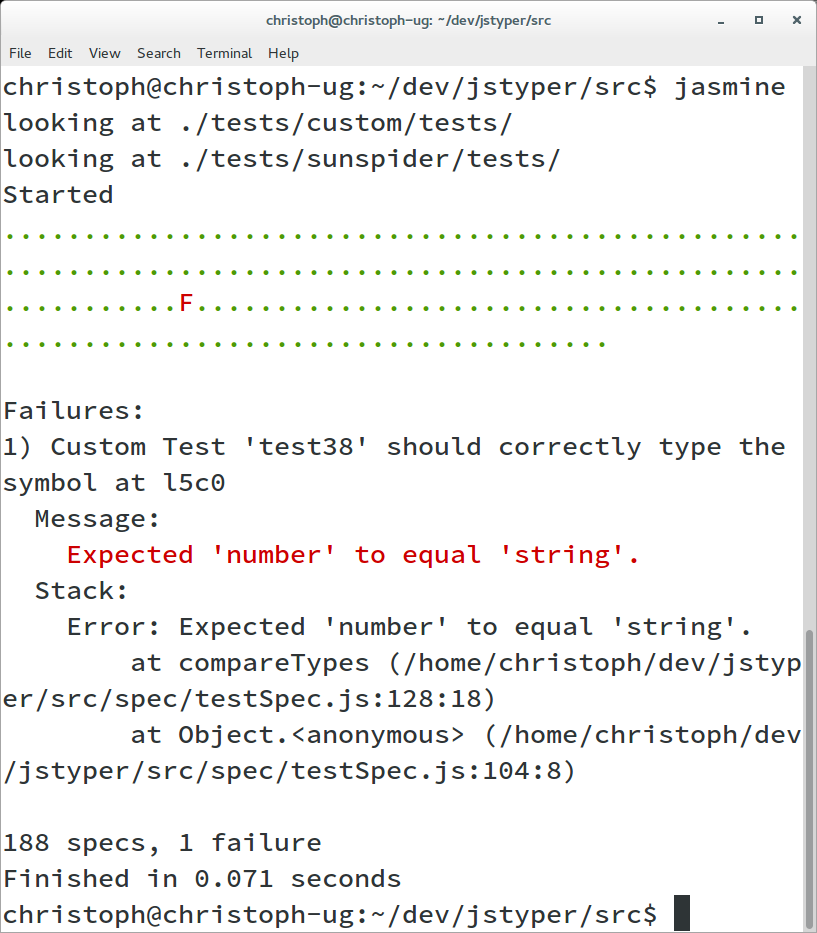
\includegraphics[width=150mm]{../res/jasmine-fail.png}}
  }
  \caption{Demonstration of the testing procedure}
  \label{fig:jasmine}
\end{figure}

In the midst of development, however, it would often be tedious to make small
modifications to several files in order to do a quick `sanity check' of
different variations on a test. To allow me to quickly carry out these informal
tests, I also built a dynamic web interface to the compiler, shown in
Figure~\ref{fig:web-interface}.  The compiler runs on the server, and the
client makes a request to recompile the input each time the user stops typing.
This gives a very responsive interface, and quickly allowed me to verify that
variations on a particular test did not introduce any new problems. When
testing the type inference, it was mainly the inserted type annotations which
were of interest. The interface was also useful when it came to testing the
gradual typing, however, as I was able to see the generated wrappers `live' as
I edited the source code. Using a web browser to do this enabled me to run both
the original and the compiled code immediately, to check that the output was
identical.

\section{Testing and Profiling the Compiler}

\subsection*{Correctness}

To test the correctness of the compiler, the test procedure outlined above was
extended. Properties were added to some JSON files, containing
key--value pairs indicating the expected value of different variables after
execution of the compiled file. The compiled file should always return the same
values as the uncompiled file, except in the case that the dynamic code
contains a type error. In this situation, the result of
uncompiled file is clearly not reliable, so we instead merely check that the
compiled code throws a cast error when executed.

Few of my unit tests performed meaningful calculations, and so judging the
correctness of these tests was not particularly enlightening. As such, I wrote
10 more representative examples of JavaScript, in order to verify that the
program result was unchanged. In half of these, a deliberate dynamic type error
was inserted, such that types were coerced in the uncompiled code, and the
original result was actually incorrect. In these 5 tests, a CastError was
correctly thrown by the \texttt{mimic} function, and the result in the other 5
tests was correctly calculated. Again, this gave me confidence in the correctness
of the compiler.

In addition to these, I ran my compiler on 5 tests from the SunSpider benchmark
suite.\footnote{https://www.webkit.org/perf/sunspider/sunspider.html} The
SunSpider suite of tests is designed to avoid `microbenchmarks', and aims to
reflect real-world use of JavaScript. This made many of the tests 
inappropriate for my purposes, since they involved manipulation of DOM objects.
Others involved object inheritance, which I was unfortunately unable to
implement before the end of the project, leaving me with relatively few to test
with. The remaining tests, however, required very little modification in order
to pass the type checker. The main
changes were syntactic (replacing \js{new Array(1,2,3)} with the literal
\js{[1,2,3]}, for example). In a few cases I left fragments unchecked, because
a language feature was unavailable. For example, my language does not
support bitwise-shift operators, but I can replace such shifts with a call to a
dynamic \js{shiftLeft} function, which is defined outside the typed world. I
employed a similar procedure to support the \js{Math} object, which is built in
to browsers, and so the type-checker cannot simply examine the definition of
\js{Math} to determine its type signature.

Since the SunSpider tests were fairly well statically typed, there were no
occasions for dynamic type errors to be thrown. With the \js{Math} object
and shift operators wrapped as described above, the correct results were
computed, and so I am confident that my gradual typing compiler is
sound.

\subsection*{Performance}

Enclosing dynamic variables within a wrapper will inevitably incur a cost both in
terms of speed and memory use. This is particularly likely to be a
problem with data of higher order types, since the contents will need
re-wrapping each time a property is read, for example. In order to evaluate the
extent of the performance hit, I analysed the runtime performance of the 10
gradual typing tests above (the tests containing cast errors were obviously
of no use here, since their execution is interrupted).

The speed of the computation was an easy measurement to make -- simply time how
long a few iterations of the test take to complete both with and without the
inserted wrappers. To measure the memory footprint, I used a plugin for Node
called \textit{memwatch}\footnote{\href{http://github.com/lloyd/node-memwatch}{http://github.com/lloyd/node-memwatch}},
to trigger heap dumps, and calculate the
difference in usage before and after the test was run. This is not an ideal
indication of memory use during the course of the test itself, since the
garbage collector may have already cleaned up some of the used memory by the
time the heap dump is triggered. More detailed analysis tools are not 
commonly available for Node, however.

\begin{figure}[H]
  \resizebox{150mm}{!}{
 	\import{../res/}{speed.pdf_tex}
  }
  \caption{Slowdown / Indirect Access \\ \footnotesize{Square tests are from the SunSpider suite}}
  \label{fig:slowdown}
\end{figure}

Figure~\ref{fig:slowdown} shows the effect on runtime speed for each test. 
There is a strong correlation between the number of indirect accesses
and the slowdown factor, which lines up with what I would expect. Each time a
property is accessed, or a function called through a wrapper, we 
introduce some overhead. I would expect this overhead to vary in size depending 
on the complexity of the item being retrieved -- a longer delay caused 
by recreating an object than by simple checking the type of a primitive. More fine-grained
analysis of the nature of the property accesses would reveal this, though a larger
set of tests would be required for this to be instructive.

Although I expected to find the same correlation between indirect accesses and
memory footprint, none was immediately apparent (Figure~\ref{fig:mem1}). My
suspicion for the cause of this was the lifespan of the wrapped objects. Since
most of the tests perform their computation in a loop, many objects have no active references
at the end of an iteration, and so the JavaScript garbage
collector can destroy these objects before creating new ones. This replacement
would not be visible when simply comparing the heap size before and after the test
is run. 

I calculated an approximate metric for the lifespan of a wrapper by dividing
the number of wrappers created by the number of indirect accesses.  This
provides an estimate for the average number of property accesses per wrapper
created. Since we would expect a longer-lived object to be used more times, we
can use this as an approximate proxy for lifespan. According to this metric,
all tests did indeed use fairly short-lived wrappers which would allow for the
kind of garbage collector optimisation discussed above. Plotting lifespan
against memory use shows a weak correlation (Figure~\ref{fig:mem2}), which may
suggest that using short-lived dynamic objects would limit the impact on
overall memory use.

\begin{figure}[H]

  \resizebox{150mm}{!}{
 	\import{../res/}{mem1.pdf_tex}
  }
  \caption{Heap Usage / Indirect Access\\ \footnotesize{Square tests are from the SunSpider suite}}
  \label{fig:mem1}
\end{figure}
\begin{figure}[H]
  \resizebox{150mm}{!}{
 	\import{../res/}{mem2.pdf_tex}
  }
  \caption{Heap Usage / Accesses per Wrapper\\ \footnotesize{Square tests are from the SunSpider suite}}
  \label{fig:mem2}
\end{figure}
Although the SunSpider tests were chosen to reflect real-world usage of
JavaScript, they present very few examples of truly dynamic behaviour.
The wrapped objects have fairly simple types (no 
more complex than a function between primitive types), and actually behave 
statically. That such code is touted as representative of
production JavaScript strengthens my belief that in practice, most programmers obey a 
static typing discipline even when the programming language itself does not enforce it.
If this is indeed the case, then any impact on runtime performance should be minimal,
as few wrappers should be required.

Another optimisation may be to reduce the number of wrappers created. Although
a function may be dynamic, it may output values which are themselves static. We
need to wrap these values in case they behave dynamically, but in reality this
is a waste of resources. We could avoid this situation by taking advantage of
the fact that my type inference system, being written in JavaScript, could
actually run within the browser. Instead of re-wrapping function return values,
it may be advantageous in some situations to perform online static analysis of
the value during program execution and avoid the need to create a new wrapper.

\chapter{Conclusions}

I have successfully achieved every objective set out in my original project
proposal.  I have precisely defined operational semantics and typing judgements
for subset of JavaScript, and my proofs of type preservation and progress
indicate that my subset was well defined.  I have implemented a type inference
system based on this specification, which passes every test in a suite of over
90 of my own tests, and several `real-world' programs from the SunSpider
benchmark suite. Finally, I have created a source-to-source compiler to
protect the statically-typed portions of a codebase from the unchecked parts. I
also achieved two of my three suggested extension tasks: the challenges of
typing arrays, and of supporting the dynamic growth of objects. In carrying the
project out, I have learned to use a range of new tools, from Ott to memwatch,
and hugely increased my understanding of types and programming languages. Some
work could yet be done to take the project further, and some ideas in this
direction are included below.

\section{Future work}

\subsection{Constraint Solution}
As indicated in chapter 3, my approach to solving constraints is not quite satisfactory. 
Although it appears functional in practice, a more rigorous approach would ensure the
soundness guarantees are preserved. Preliminary investigation into the work of
Fran\c{c}ois Pottier~\cite{pottier1998type} indicates that his approach may be of use here.

\subsection{Language Features}

Support of more language features would make the inference tool immediately
able to type a much larger set of existing JavaScript programs. One of the main
such features is prototypal inheritance. In JavaScript, each object has a
special \js{prototype} property, which corresponds to the object's parent in
the inheritance chain. Property accesses may retrieve the value from the
object itself if present, or from the object prototype if not. I believe my 
system of origin chains could be extended to support this method of inheritance 
in a straightforward manner by adding the prototype object's type as the origin
for the descendant object.

Another feature which may be useful is the inclusion of union types.
Since JavaScript has no explicit mechanism for overloading, it is common for
functions to be called with parameters of variable types. The function then
inspects the types of the arguments provided and dispatches them to the
appropriate logic. Currently such functions are excluded by the
static type system, but it would be possible to keep track of the parameters
as having a union type, which could then be discharged by explicit type checks.
This would also enable the type inference of variadic functions, which in effect
have parameters which sometimes take the value `\js{undefined}.'

\subsection{Fine-grained object modification}

Currently I am able to handle the dynamic addition of properties to objects. 
Although the monotonic growth of objects makes analysis easier, property deletion
can be quite common in some programs.~\cite{JSBehaviour} It may also be possible
to use control flow analyses to allow modification of property types, although
in practice allowing this behaviour may negate many of the benefits of the type system, which 
would normally interpret an attempt to change a property's type as a potential bug.

\section{Final Thoughts}

Although statically typing a dynamically typed programming language may appear
to be like fitting a square peg in a round hole, in practice my approach has
been successful. The additional safety guarantees which can be offered about
such statically typed programs are valuable, and future integration within code
intelligence tools could offer even greater benefits to JavaScript developers.
The process has been instructive from start to finish, and I hope to pursue the
ideas formed here further in future.

\printbibliography{}

\end{document}
